
% This is the main file to setup the document.
% Document organization and appearance settings are all done here
% Each chapter is a seate tex file, all linked together here


% Preamble (document settings) -----------------------------------------------------------
% Document type and font --
\documentclass[12pt]{article}
\usepackage[utf8]{inputenc} %utf-8 encoding for ASCII symbols

% insert packages here --
\usepackage{graphicx}       %for handling images

\usepackage{amsmath}        %for math symbols

\usepackage{breakcites}     %to avoid citations extending into the margin

\usepackage[margin=1in]{geometry}   %to reduce margins to 1 inch, default margins wasted a lot of space

\usepackage{sidecap}        %to enable side captions on figures

\usepackage{setspace}       %to enable doublespacing   
\usepackage{mathrsfs}
\usepackage{arev} %was calligra
\usepackage[T1]{fontenc}
\usepackage[none]{hyphenat}
\usepackage{float}
\usepackage{xcolor}
\usepackage[colorlinks]{hyperref}
\hypersetup{
colorlinks=true,
linkcolor=red,
urlcolor=cyan,
}
\usepackage{caption}
\usepackage{subcaption}

% http://www.mathworks.com/matlabcentral/fileexchange/8015-m-code-latex-package
\usepackage[framed,numbered,autolinebreaks,useliterate]{mcode}

\usepackage[
backend=biber,
style=apa,
citestyle=apa
]{biblatex}       %use the biblatex package

\addbibresource{mybibfile1.bib}   %path to the bib file
\addbibresource{mybibfile2.bib}


\usepackage{hyperref}       % to create a linked table of contents
\hypersetup{
    colorlinks,
    citecolor=black,
    filecolor=black,
    linkcolor=black,
    urlcolor=black
}

% Set path to images
\graphicspath{ {images/} }  % Direct to the main image folder, always good to create sub-folders to organize images for individual chapters

\singlespacing  %making text double spaces

% End of preamble
%-------------------------------------------------------------------------------------------
\begin{document}

% Making title page
%!TeX root = ../main.tex

\begin{titlepage}
   \begin{center}
   \begin{doublespacing}

       \begin{figure}
       \centering
       
\includegraphics[width=0.8\textwidth]{images/logo.png}
       \end{figure}
       
       \vspace*{10mm}
       {\large\textbf{Academic Year 2020/2021}}
       
       
       \vspace{10mm}
       {\large\textbf{Master Degree in ICT for Internet and Multimedia}\\
       \vspace{10mm}
       \textbf{02 $\cdot$ 2021}}

       
       
       \vspace*{5mm}
       {\Large\textbf{3D AUGMENTED REALITY}}

       %\textbf{DOCTOR OF PHILOSOPHY}
       \vspace{30mm}
       
       {\Large\textbf{PROJECT REPORT - B.2}}

    
            
       \vspace{30mm}

       {\large\textbf{Casagrande Nicola - De Toni Alberto}\\
       \textbf{1242363 - 1236657}}

       \vfill
              
    \end{doublespacing}

   \end{center}
\end{titlepage}


% Starting frontmatter:
% Abstract goes here
\doublespacing
% \thispagestyle{plain}
\begin{center}
    \Large
    \textbf{This is my report title}
        
    \vspace{0.4cm}
    \textbf{Claude Shannon}
    
    \vspace{0.4cm}
    \large{Supervisor: Asst/ Prof John von Neumann  }
       
    \vspace{0.9cm}
    \textbf{Abstract}
\end{center}

Abstract text goes here.. 

\pagenumbering{roman}   % Roman page numbering to start from abstract onwards

\singlespacing          % keep pre-content single spaced
%\listoffigures          % generate list of figures
%\listoftables           % generate list of tables

% End of frontmatter

% Insert table of contents
 %\tableofcontents

% Main matter starts here --
% Inserting individual chapters. Mention chapter titles here and simple link the chapter's tex file

 %\chapter{Introduction}     % Mention chapter title here
 \pagenumbering{arabic}    % We want Arabic numerals for main matter page numbering
 %!TeX root = ../main.tex

{\raggedright\large\textbf{Local feature compression using autoencoders - SfM tests}}\smallskip \\ 
Design a compression strategy for local SURF descriptors using autoencoders. Training data can be generated using the images of dataset Portello and Castle. Testing must be done on dataset FountainP-11 and Tiso (available at \url{https://github.com/openMVG/SfM_quality_evaluation/tree/master/Benchmarking_Camera_Calibration_2008} and \url{http://www.dei.unipd.it/~sim1mil/materiale/3Drecon/}). Software must be implemented in MATLAB, Keras or Pytorch. \\ \textbf{Testing on 3D reconstruction using SfM:} The reconstructed descriptors (only for the test set) are used to perform a SfM reconstruction using COLMAP (using the two test dataset). \\
Programming languages: MATLAB/Python/C++.

\section{Introduction}

\subsection{Descriptors in general}
In computer vision, visual descriptors or image descriptors are descriptions of the visual features of the contents in images, videos, or algorithms or applications that produce such descriptions. They describe elementary characteristics such as the shape, the color, the texture or the motion, among others\footnote{\url{https://en.wikipedia.org/wiki/Visual_descriptor}, 01/02/21}. A feature detector (\emph{extractor}) is an algorithm taking an image as input and outputting a set of regions (``local features'' = ``Interest Points'' = ``Keypoints'' = ``Feature Points''). A descriptor is computed on an image region defined by a detector. The descriptor is a representation of the image function (colour, shape, ...) in the region (typically an array). Two key operations are related to feature extraction:
\begin{itemize}
\item Feature detection: extract the features of interest
\item Feature description: associate a descriptor to each feature in order to distinguish from the others
\end{itemize}
There are many pre-defined descriptors available to the users. Some of them are reported in fig.\ref{fig:descriptors}.

\begin{figure}[h!]
    \centering
    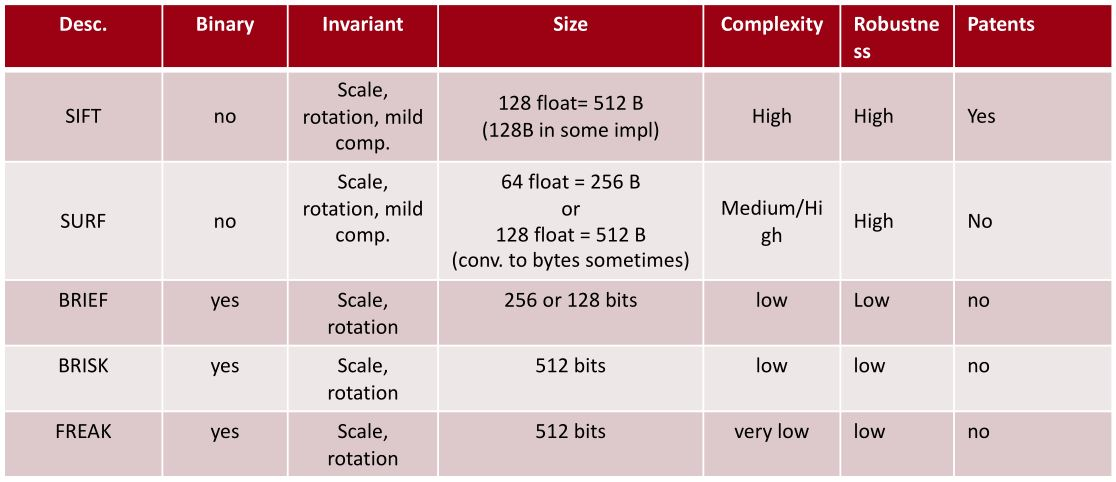
\includegraphics[width=0.9\textwidth]{images/Descriptors.jpg}
    \caption{Common algorithms for feature description.}
    \label{fig:descriptors}    
\end{figure}


\subsection{Speeded Up Robust Features (SURF)}
In computer vision, Speeded Up Robust Features (SURF) is a local feature detector and descriptor. It can be used for tasks such as object recognition, image registration, classification, or 3D reconstruction. It is partly inspired by the Scale-Invariant Feature Transform (SIFT) descriptor. The standard version of SURF is several times faster than SIFT and claimed by its authors to be more robust against different image transformations than SIFT\footnote{\url{https://https://https://en.wikipedia.org/wiki/Speeded_up_robust_features}, 01/02/21}. The SURF algorithm is based on three main parts:
\begin{itemize}
\item Detection: using a blob detector method based on the Hessian matrix to find feature points
\item Description: the goal of a descriptor is to provide a unique and robust description of an image feature
\item Matching: comparing the descriptors obtained from different images to find the matching pairs
\end{itemize}



\subsection{Autoencoders in general}
An autoencoder is a type of artificial neural network used to learn efficient data codings in an unsupervised manner. The aim of an autoencoder is to learn a representation (encoding) for a set of data, typically for dimensionality reduction, by training the network to ignore signal “noise”. Along with the reduction side, a reconstructing side is learnt, where the autoencoder tries to generate from the reduced encoding a representation as close as possible to its original input\footnote{\url{https://https://en.wikipedia.org/wiki/Autoencoder}, 01/02/21}.
There are two categories of autoencoder:
\begin{itemize}
\item Regularized autoencoders: they are divided into three types such as Sparse autoencoder (SAE), Denoising autoencoder (DAE) and Contractive autoencoder (CAE)
\item Variational autoencoders (VAE): generative models akin to generative adversarial networks (GAN)
\end{itemize}
A basic autoencoder as shown in fig. \ref{fig:autoencoder}  has an internal hidden layer and it's made of two main parts which are the encoder that turns a high-dimensional input into a latent low-dimensional code, and the decoder that performs a reconstruction of the input with this latent code. It's also possible to train the autoencoder with multiple layers to exponentially reduce the computational cost of representing some functions and to exponentially decrease the amount of training data needed to learn some functions. 
The two steps of using an autoencoder are:
\begin{itemize}
\item Training
\item Testing
\end{itemize}
\begin{figure}[h!]
    \centering
    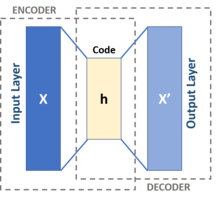
\includegraphics[width=0.4\textwidth]{images/autoencoder.png}
    \caption{Scheme of a basic autoencoder.}
    \label{fig:autoencoder}    
\end{figure}

\subsection{Development software}
MATLAB is a proprietary multi-paradigm programming language and numeric computing environment developed by MathWorks. MATLAB allows matrix manipulations, plotting of functions and data, implementation of algorithms, creation of user interfaces, and interfacing with programs written in other languages\footnote{\url{https://https://https://https://en.wikipedia.org/wiki/MATLAB}, 02/02/21}. We decided to use Matlab as Machine Learning tool because we felt more confident, while also it has an extensive documentation and it offers different advantages:
\begin{itemize}
\item Implement and test algorithms easily
\item Develop the computational codes easily
\item Debug easily
\item Use a large database of built in algorithms
\item Process still images and create simulation videos easily
\item Symbolic computation can be easily done
\item Possibility of calling external libraries
\item Perform extensive data analysis and visualization
\item Develop application with graphics user interface
\end{itemize}


\subsection{Goal of the project}
The objective of the project is to develop a compression strategy for local SURF descriptors using an autoencoder and perform a SfM reconstruction using COLMAP software with the obtained data. The matchings and the features must be saved in a .txt file. The autoencoder has to be trained with training data generated from a given dataset and has to be tested on another dataset. The final result should display a worse reconstruction due the compression of the data and the goal is to find a good setting for the autoencoder.  % Link to the chapter tex file


%\chapter{Some Literature review}
%!TeX root = ../main.tex

\section{Data}
The data of the experiment are divided into two groups of images, one used for the training of the autoencoder and another one for the testing. The images represent four architectural elements from different points of view. In the training group there are images of Portello and Castle (some of them are reported in fig. \ref{fig:portello} and fig. \ref{fig:castle}), while in the group of the testing images there are images of fountain and Tiso, some of them reported in fig. \ref{fig:fountain} and fig. \ref{fig:tiso}.

\begin{figure}[H]
     \centering
     \begin{subfigure}[b]{0.3\textwidth}
         \centering
         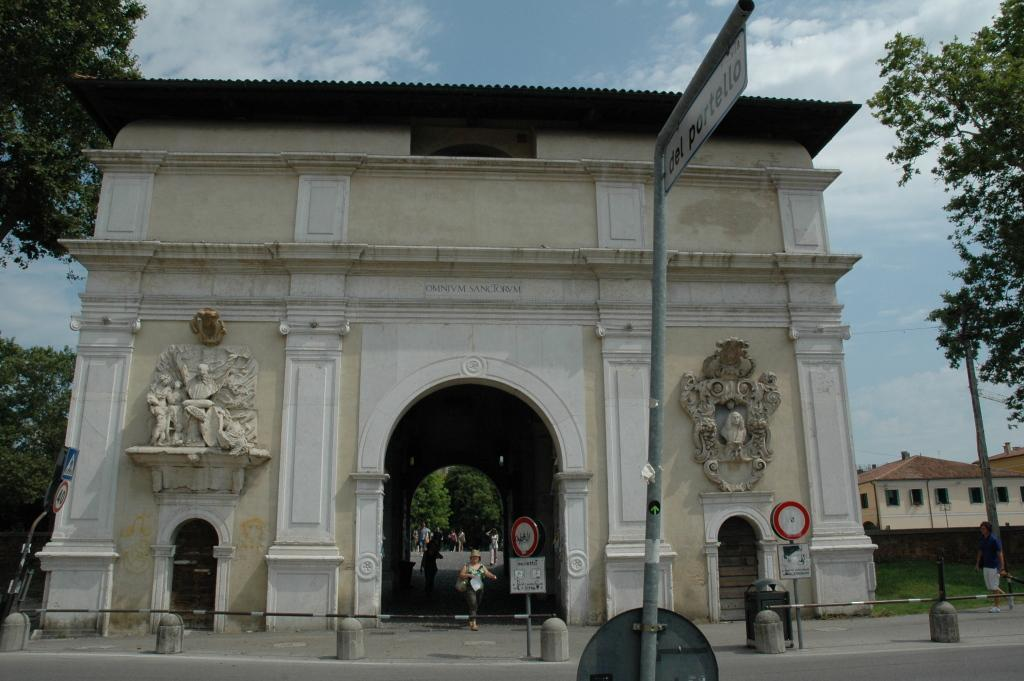
\includegraphics[width=\textwidth]{../../Project_3DAR/images/Training/portelloDataset/img000.jpg}
     \end{subfigure}
     \hfill
     \begin{subfigure}[b]{0.3\textwidth}
         \centering
         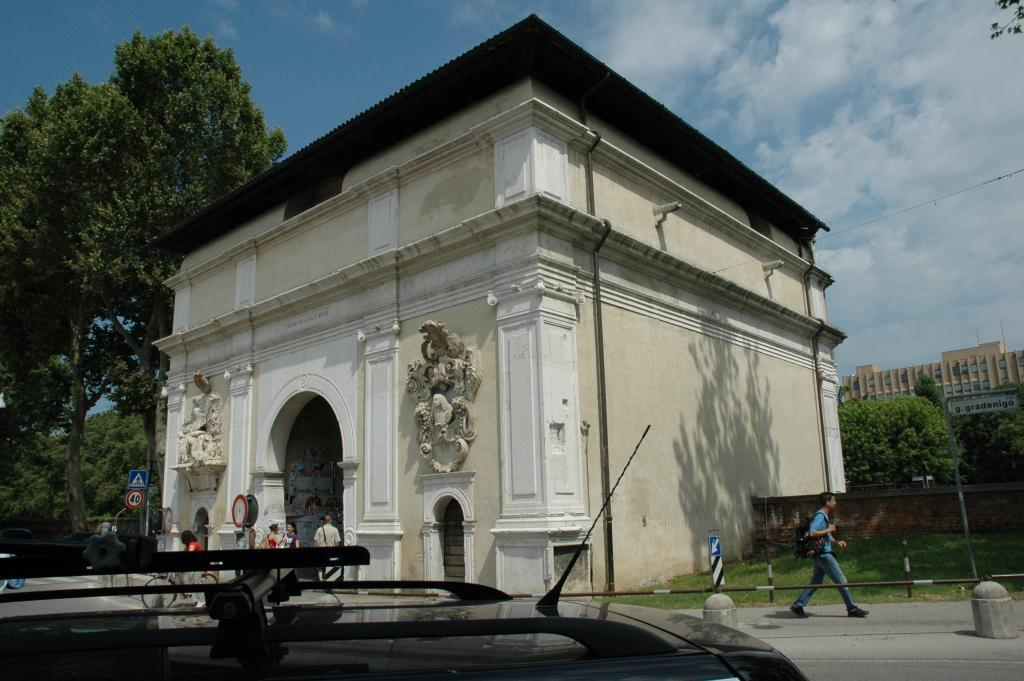
\includegraphics[width=\textwidth]{../../Project_3DAR/images/Training/portelloDataset/img013.jpg}
     \end{subfigure}
     \hfill
     \begin{subfigure}[b]{0.3\textwidth}
         \centering
         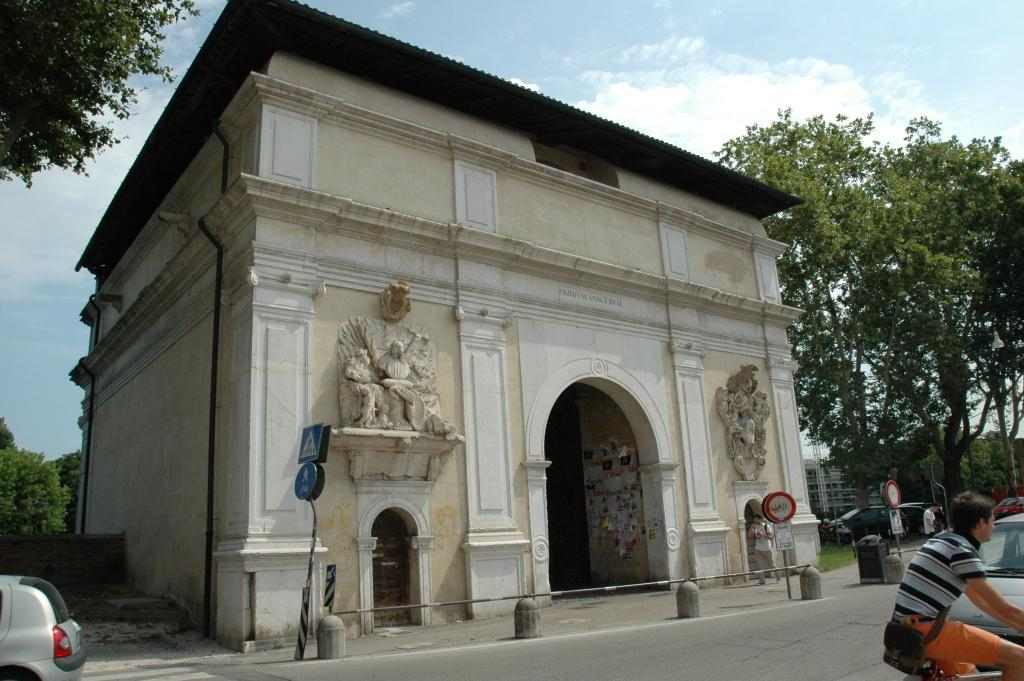
\includegraphics[width=\textwidth]{../../Project_3DAR/images/Training/portelloDataset/img030.jpg}
     \end{subfigure}
        \caption{samples from Portello dataset.}
        \label{fig:portello}
\end{figure}

\begin{figure}[H]
     \centering
     \begin{subfigure}[b]{0.3\textwidth}
         \centering
         \includegraphics[width=\textwidth]{../../Project_3DAR/images/Training/castle/0004.jpg}
     \end{subfigure}
     \hfill
     \begin{subfigure}[b]{0.3\textwidth}
         \centering
         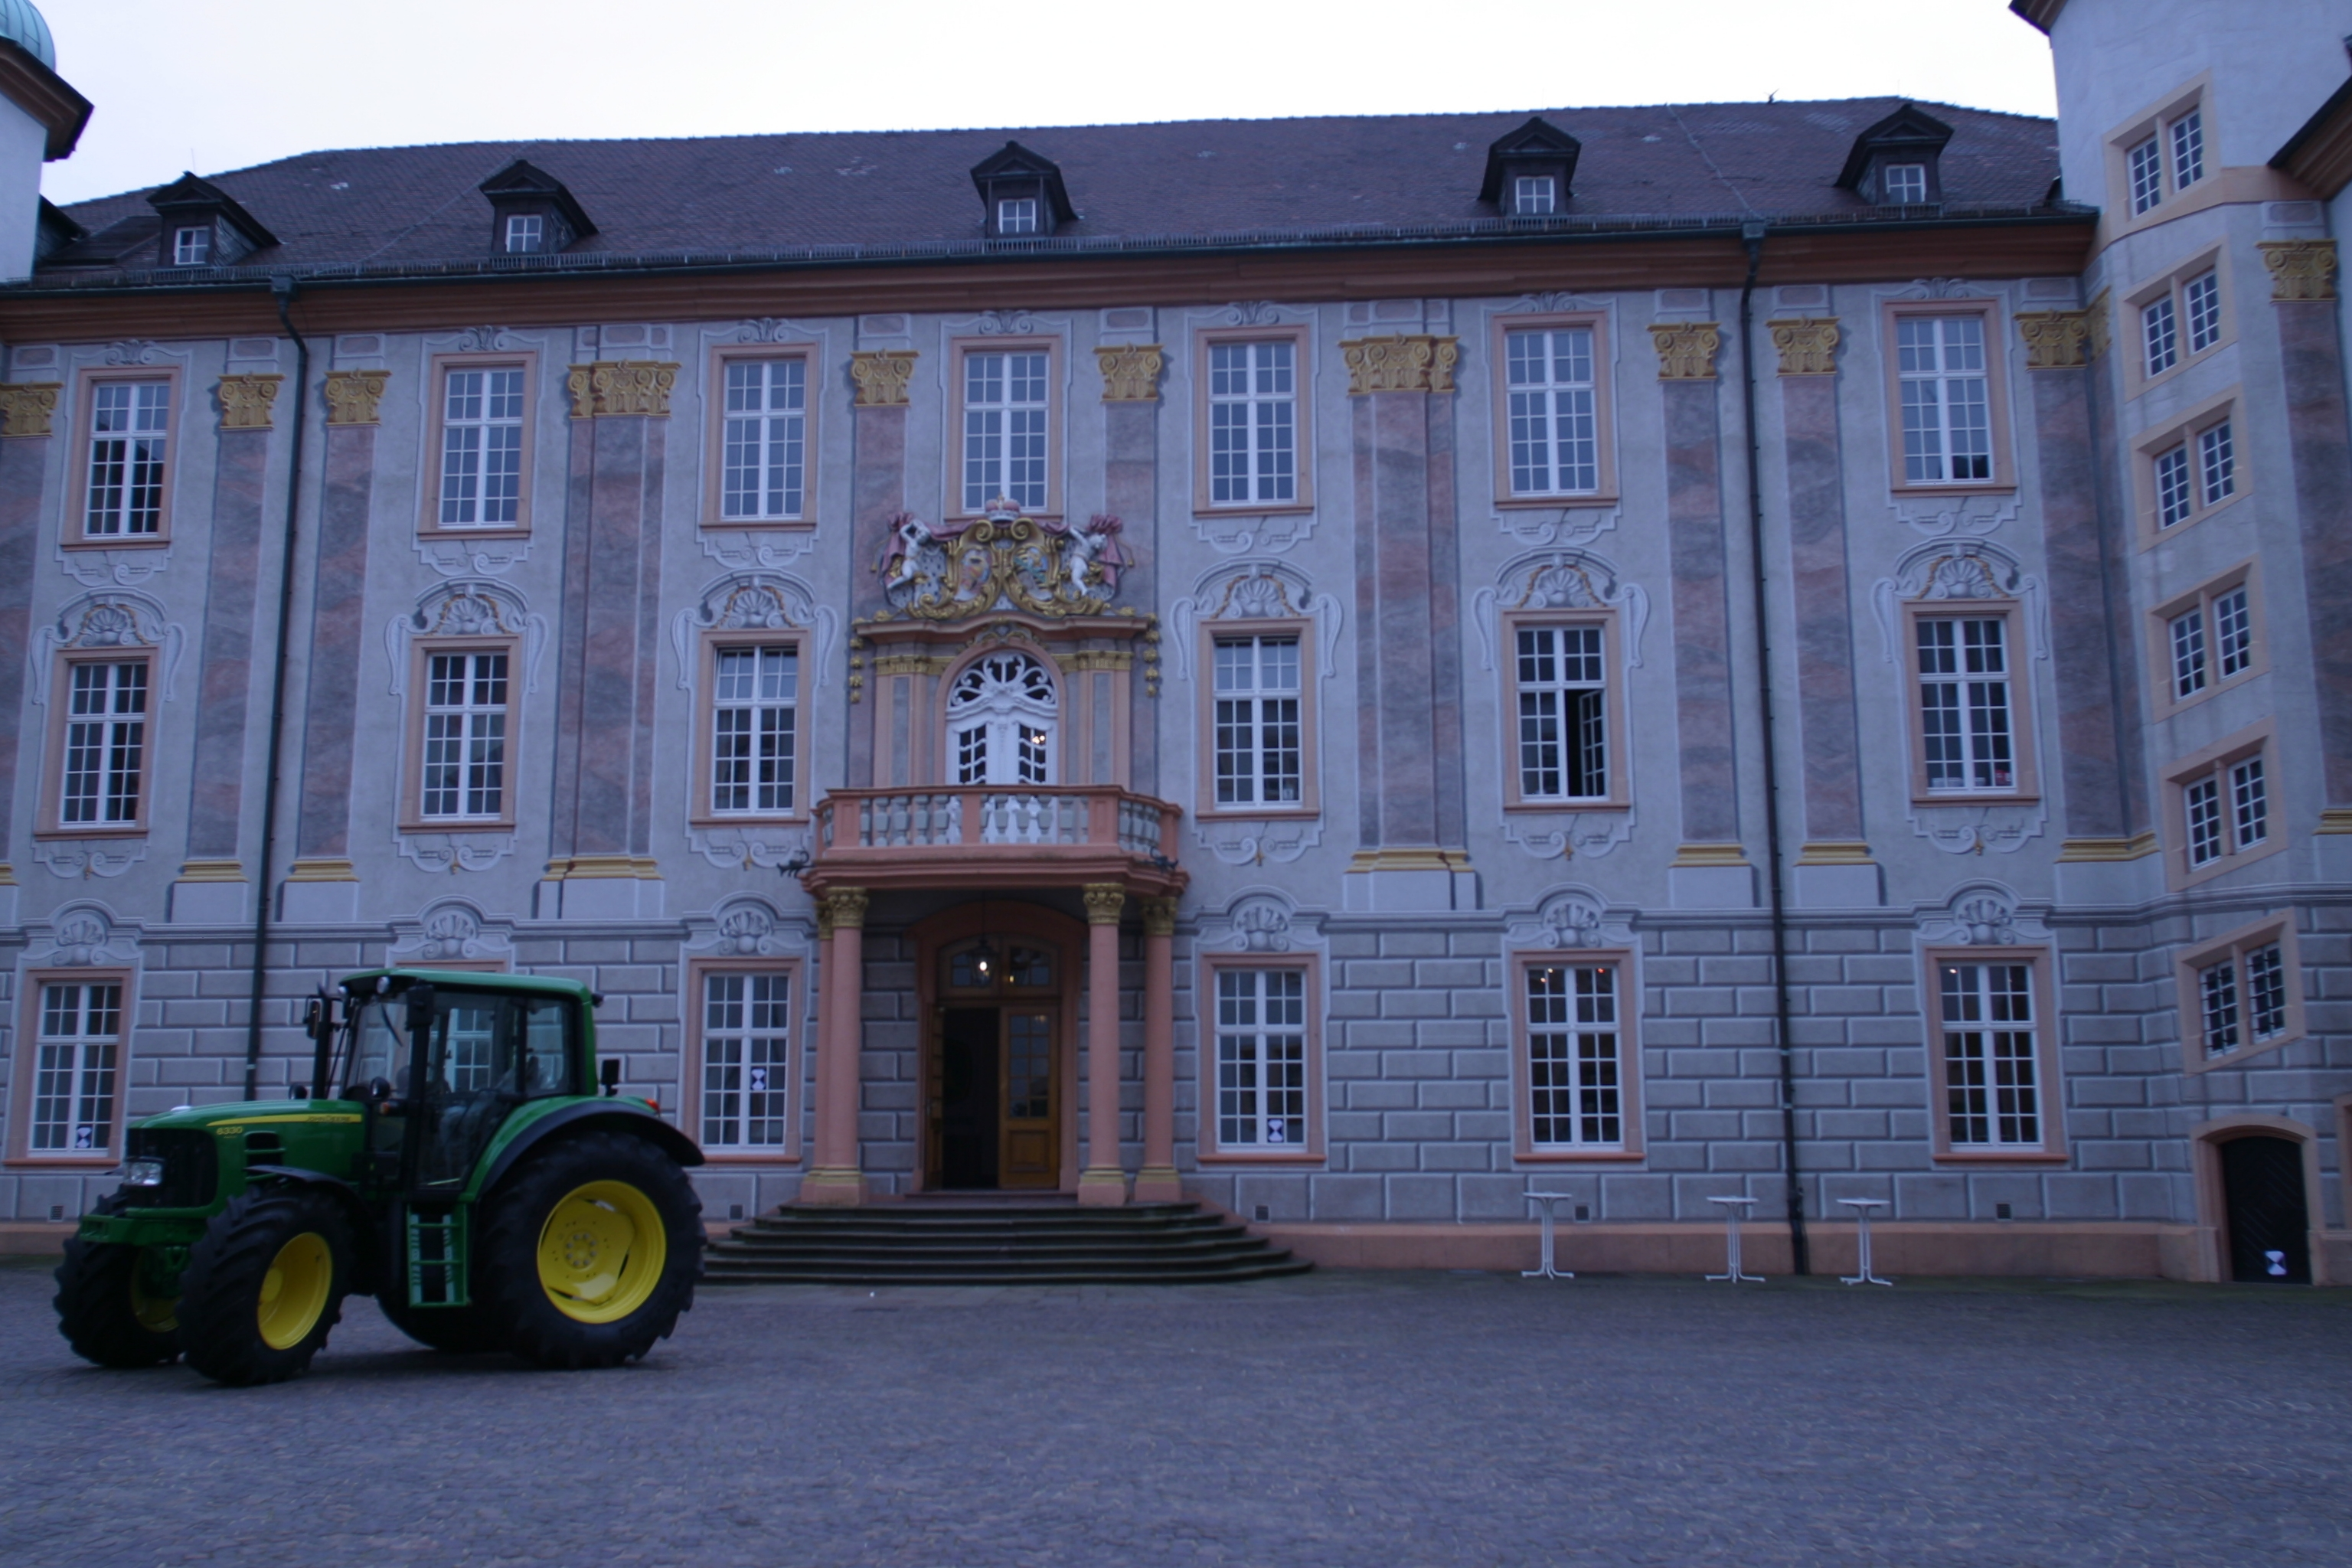
\includegraphics[width=\textwidth]{../../Project_3DAR/images/Training/castle/0010.jpg}
     \end{subfigure}
     \hfill
     \begin{subfigure}[b]{0.3\textwidth}
         \centering
         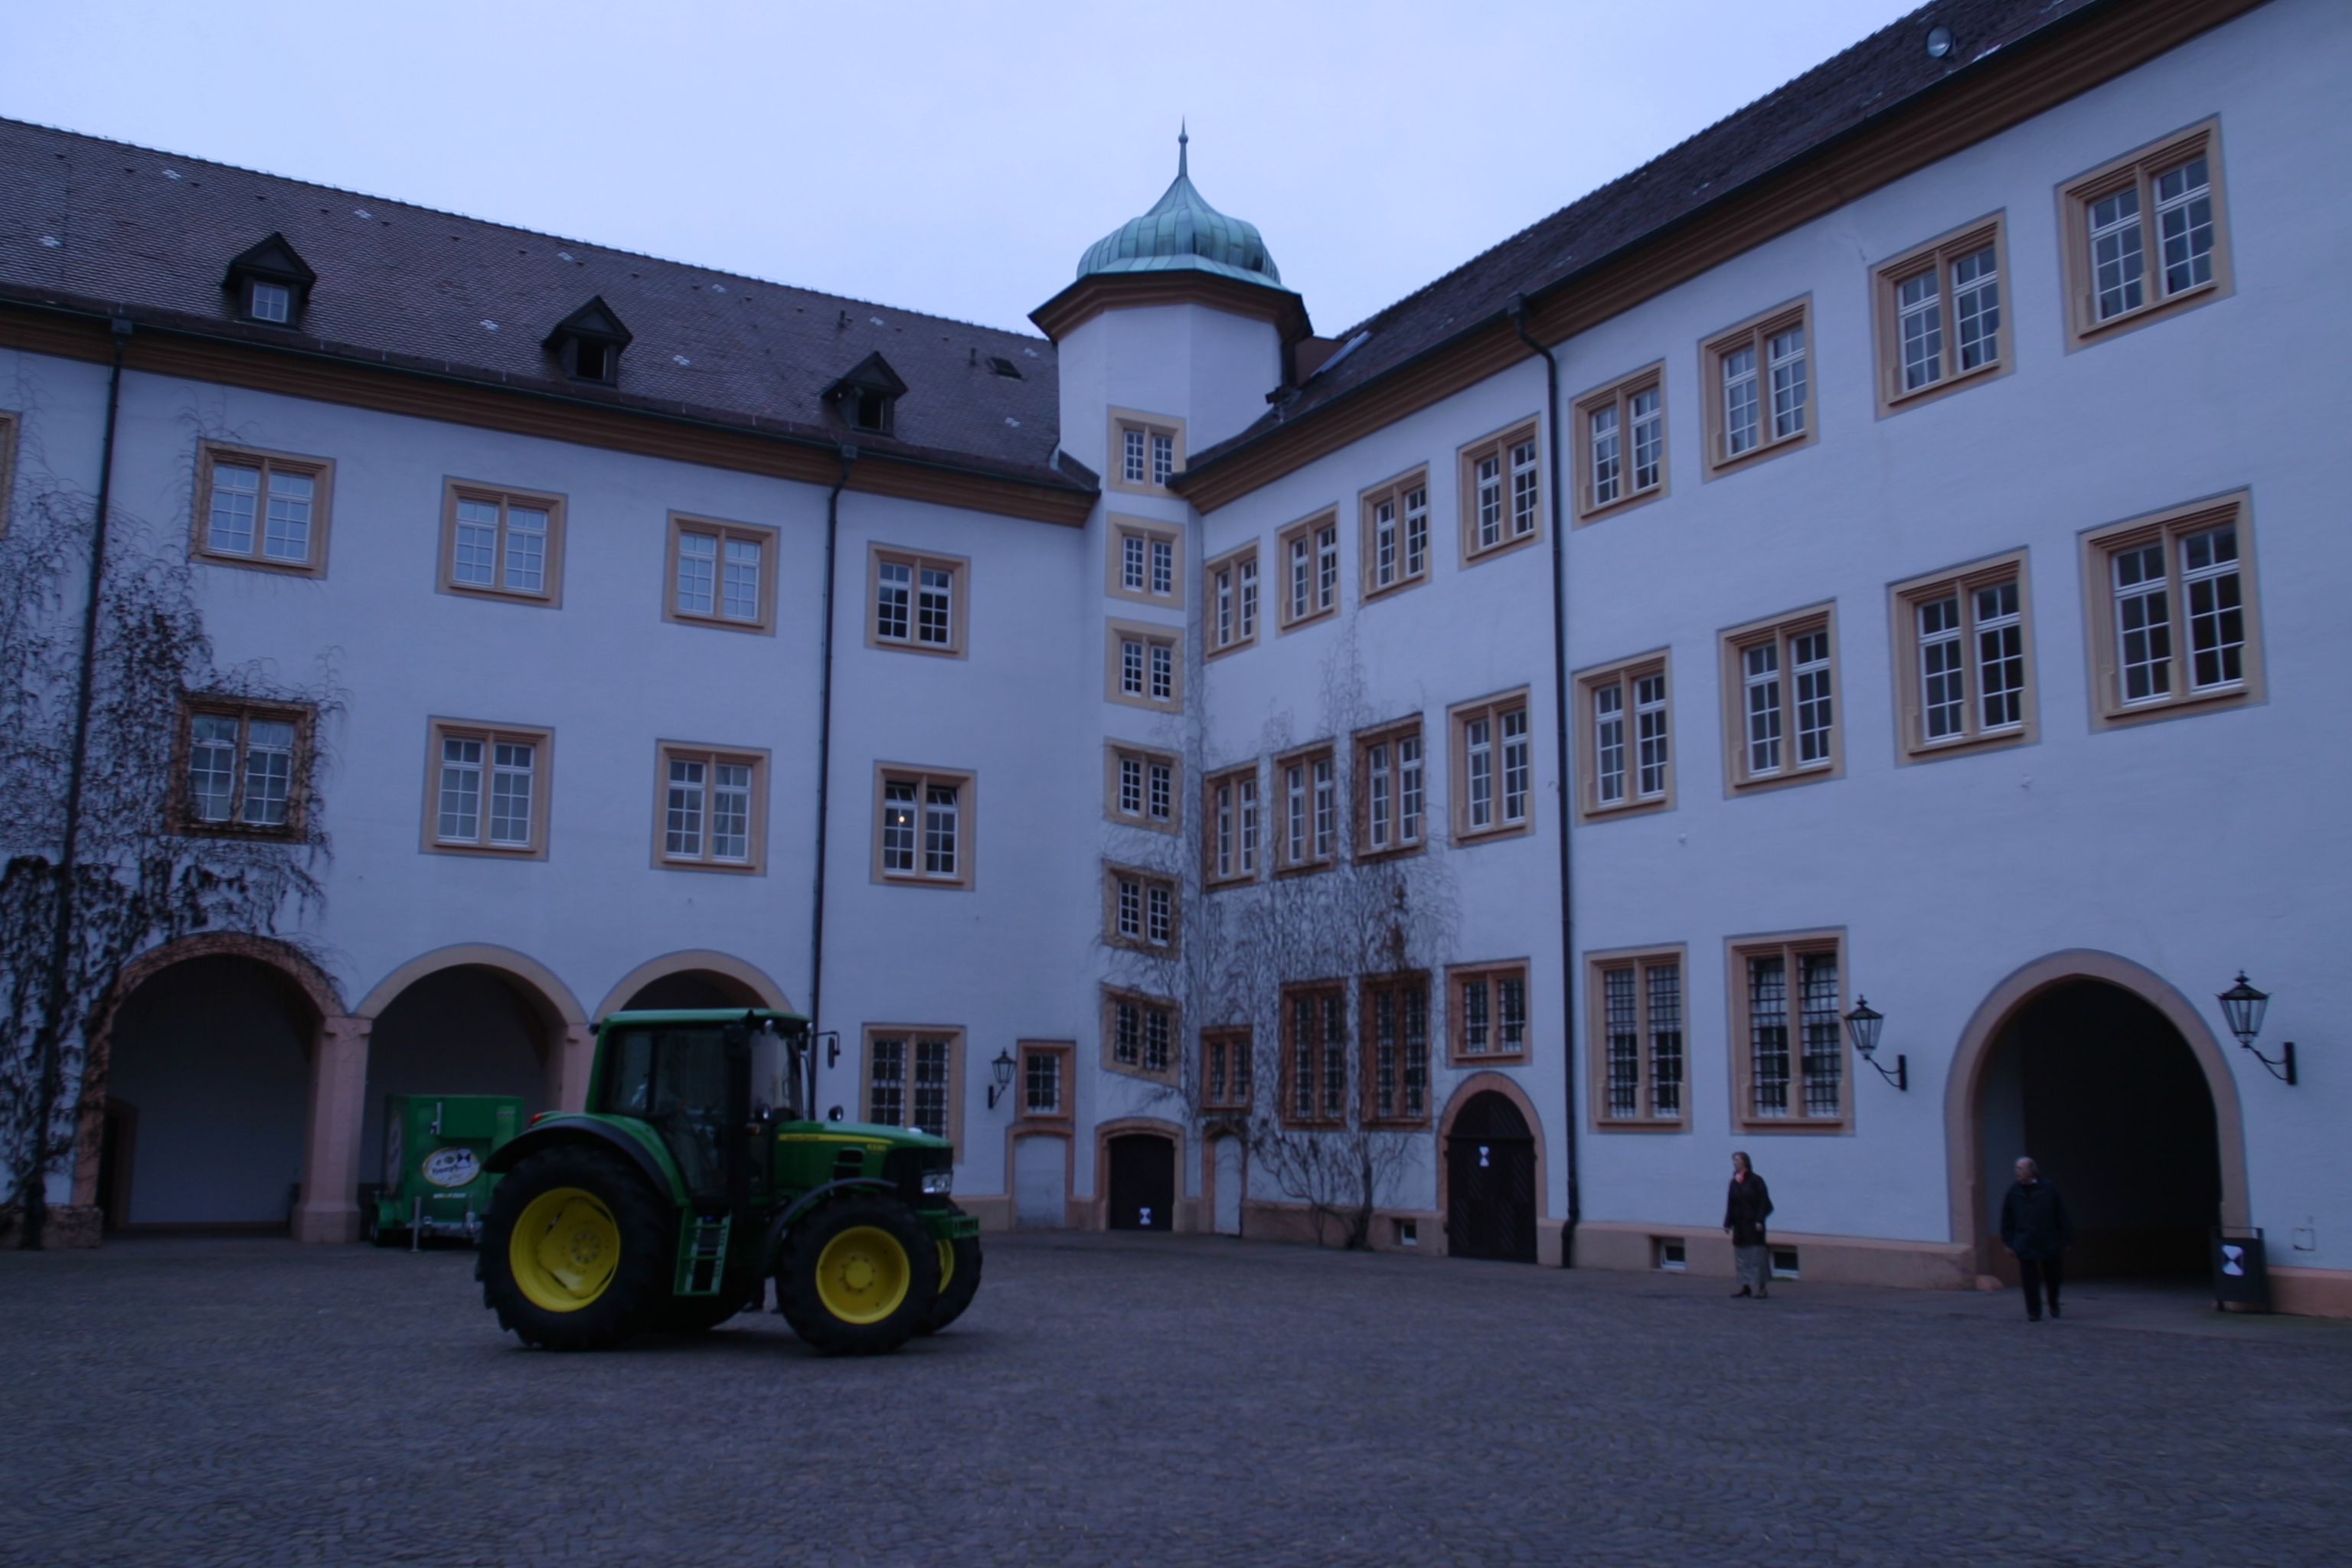
\includegraphics[width=\textwidth]{../../Project_3DAR/images/Training/castle/0028.jpg}
     \end{subfigure}
        \caption{samples from castle dataset.}
        \label{fig:castle}
\end{figure}

\begin{figure}[H]
     \centering
     \begin{subfigure}[b]{0.3\textwidth}
         \centering
         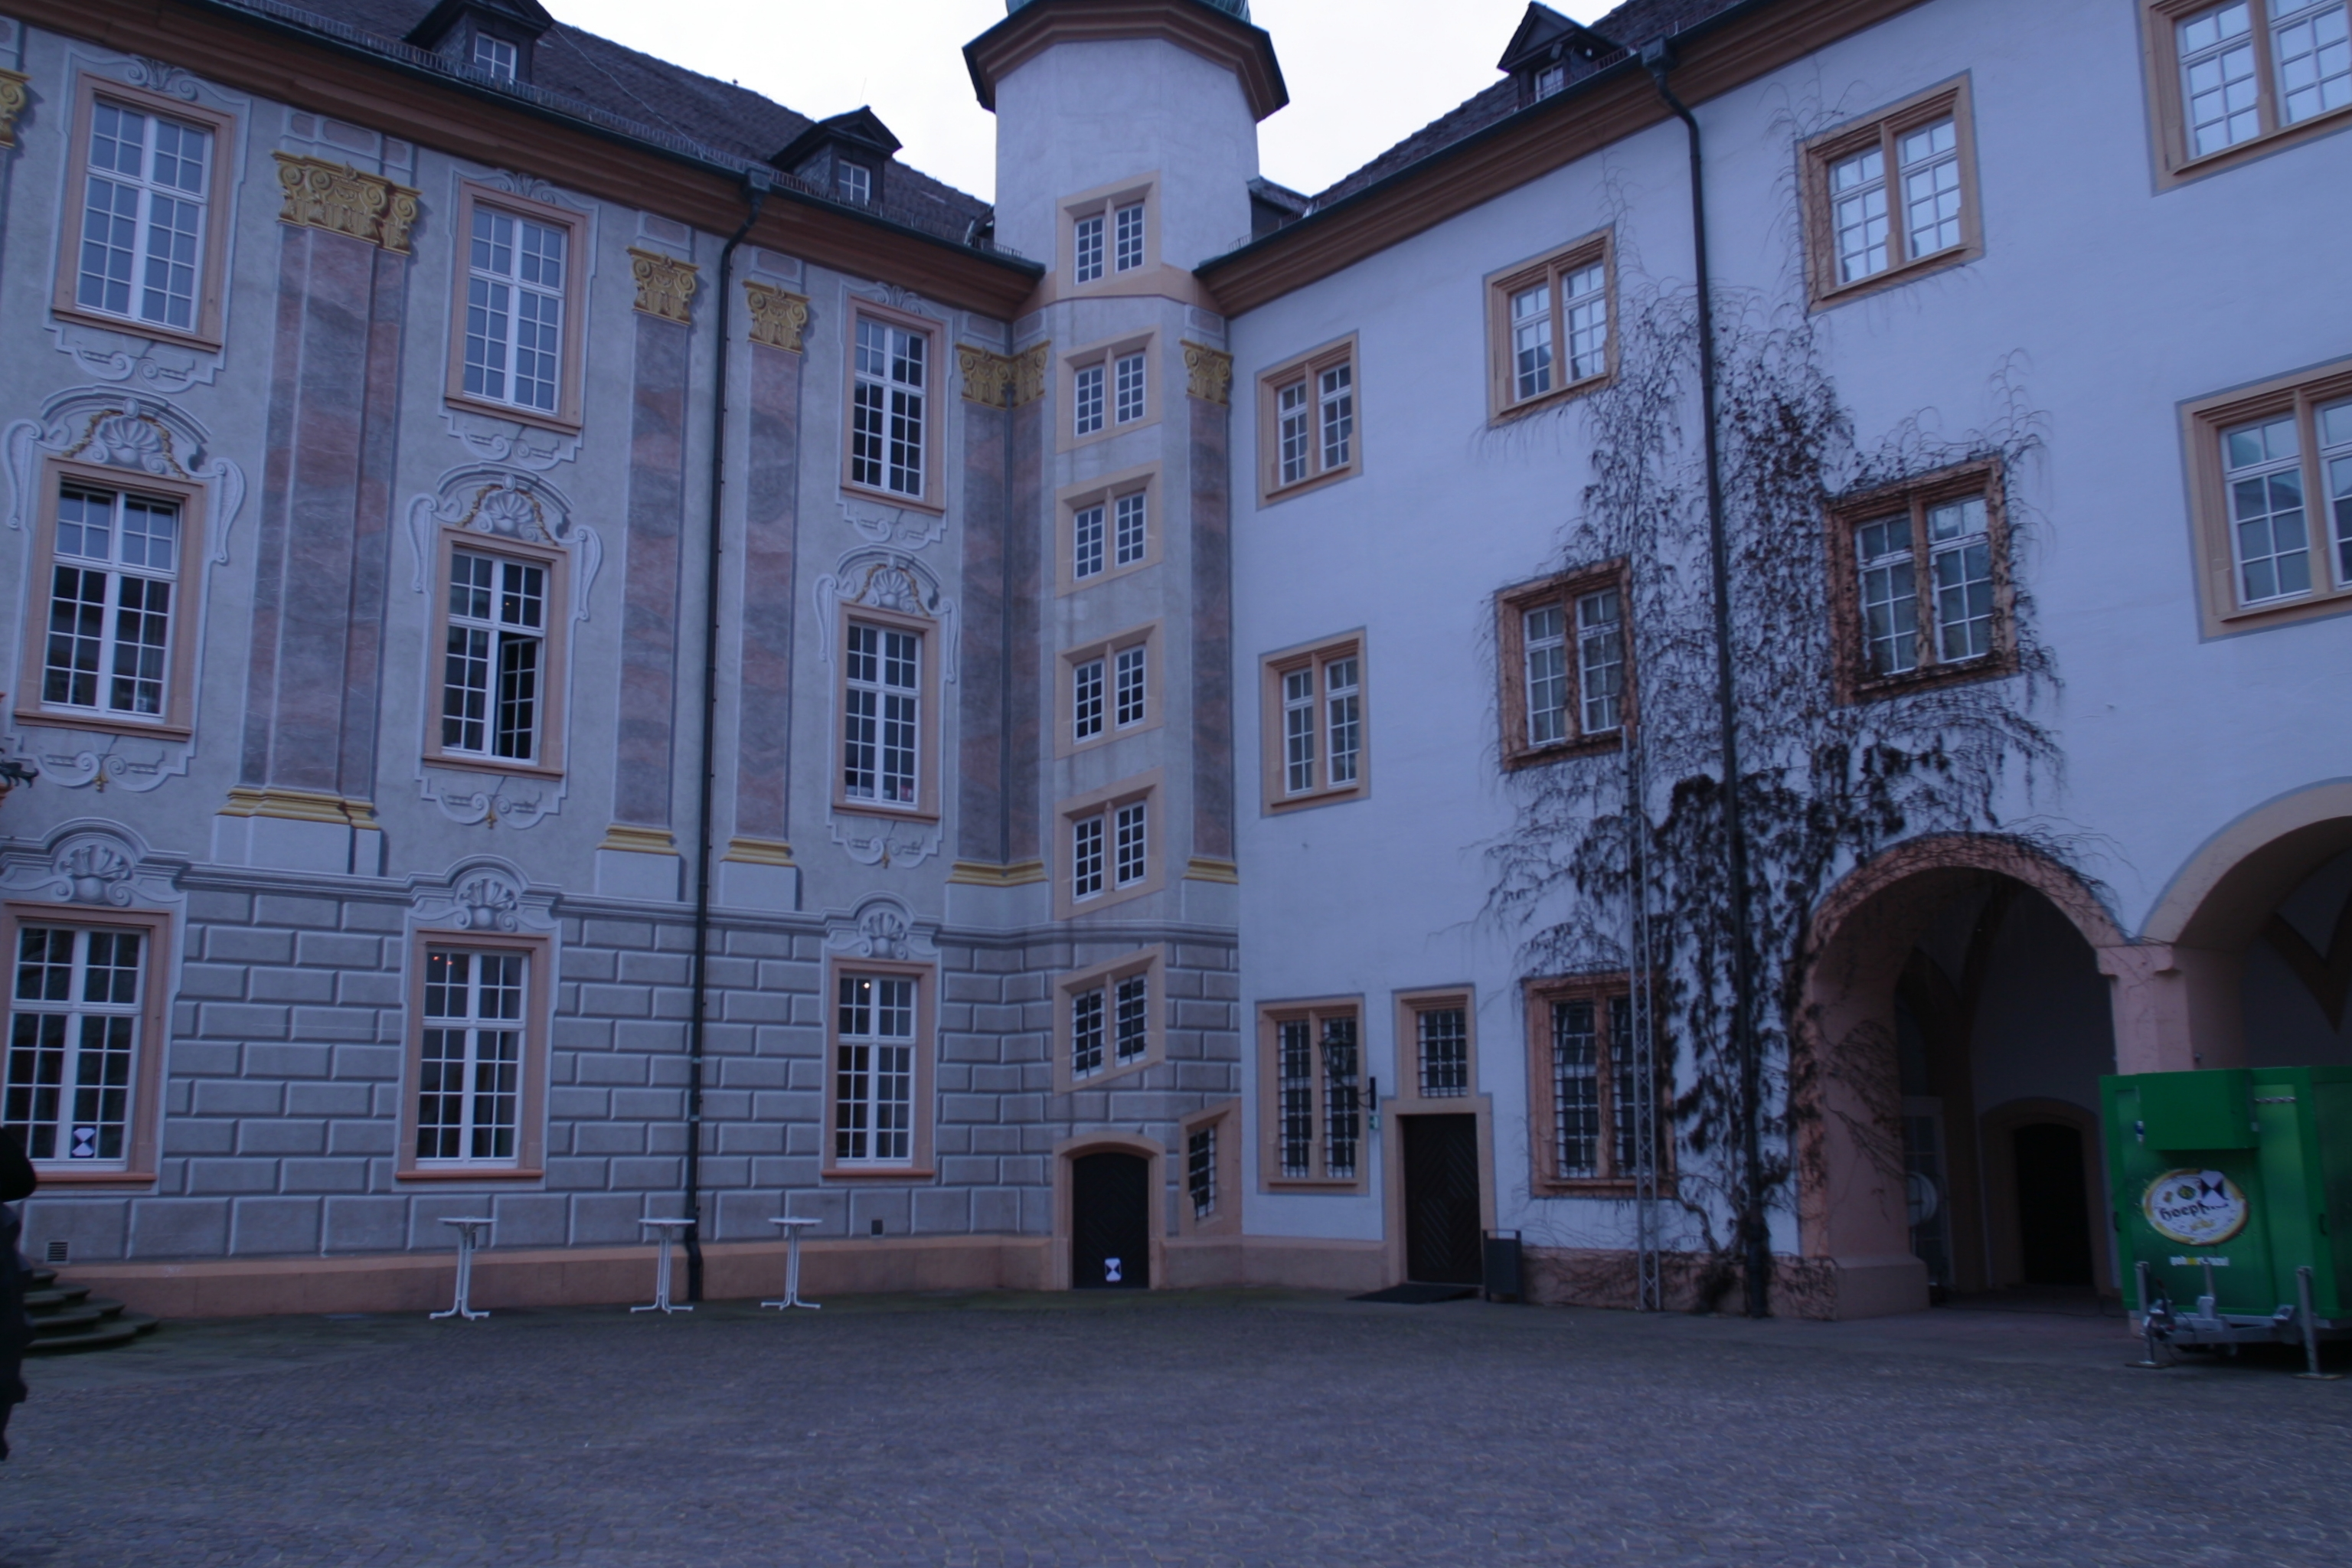
\includegraphics[width=\textwidth]{../../Project_3DAR/images/Testing/fountain-P11/0000.jpg}
     \end{subfigure}
     \hfill
     \begin{subfigure}[b]{0.3\textwidth}
         \centering
         \includegraphics[width=\textwidth]{../../Project_3DAR/images/Testing/fountain-P11/0004.jpg}
     \end{subfigure}
     \hfill
     \begin{subfigure}[b]{0.3\textwidth}
         \centering
         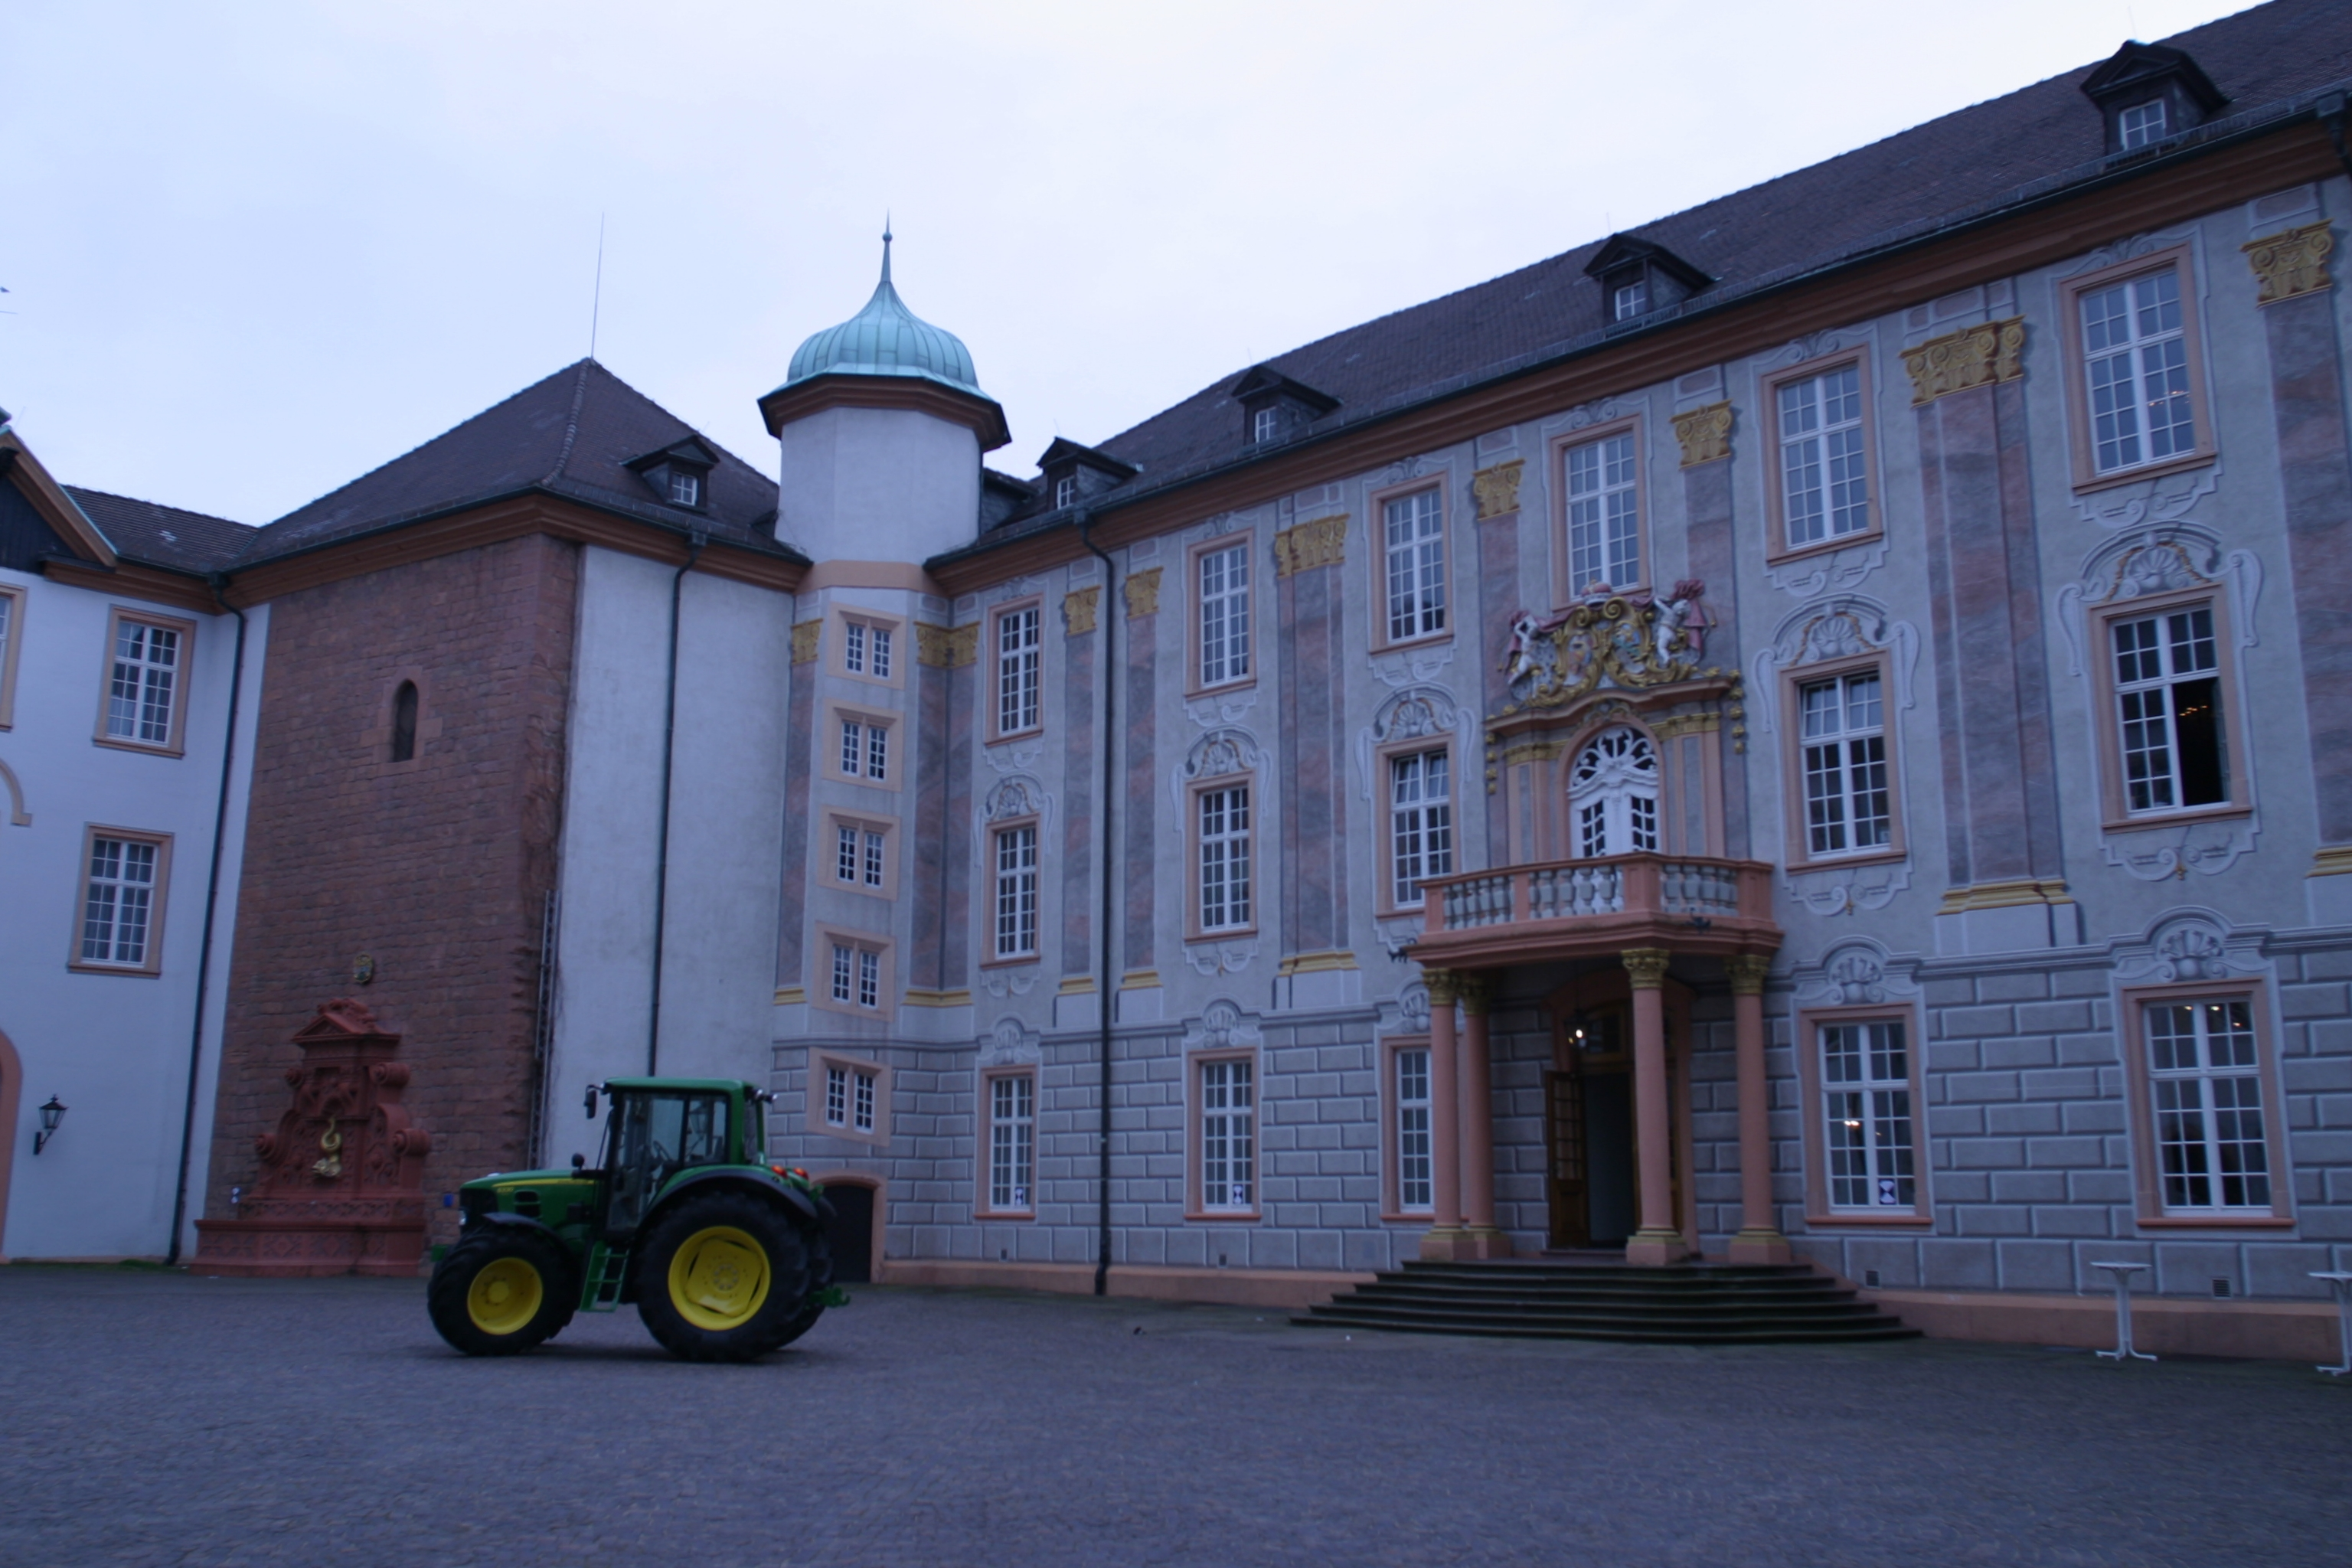
\includegraphics[width=\textwidth]{../../Project_3DAR/images/Testing/fountain-P11/0008.jpg}
     \end{subfigure}
        \caption{samples from Fountain-P11 dataset.}
        \label{fig:fountain}
\end{figure}

\begin{figure}[H]
     \centering
     \begin{subfigure}[b]{0.3\textwidth}
         \centering
         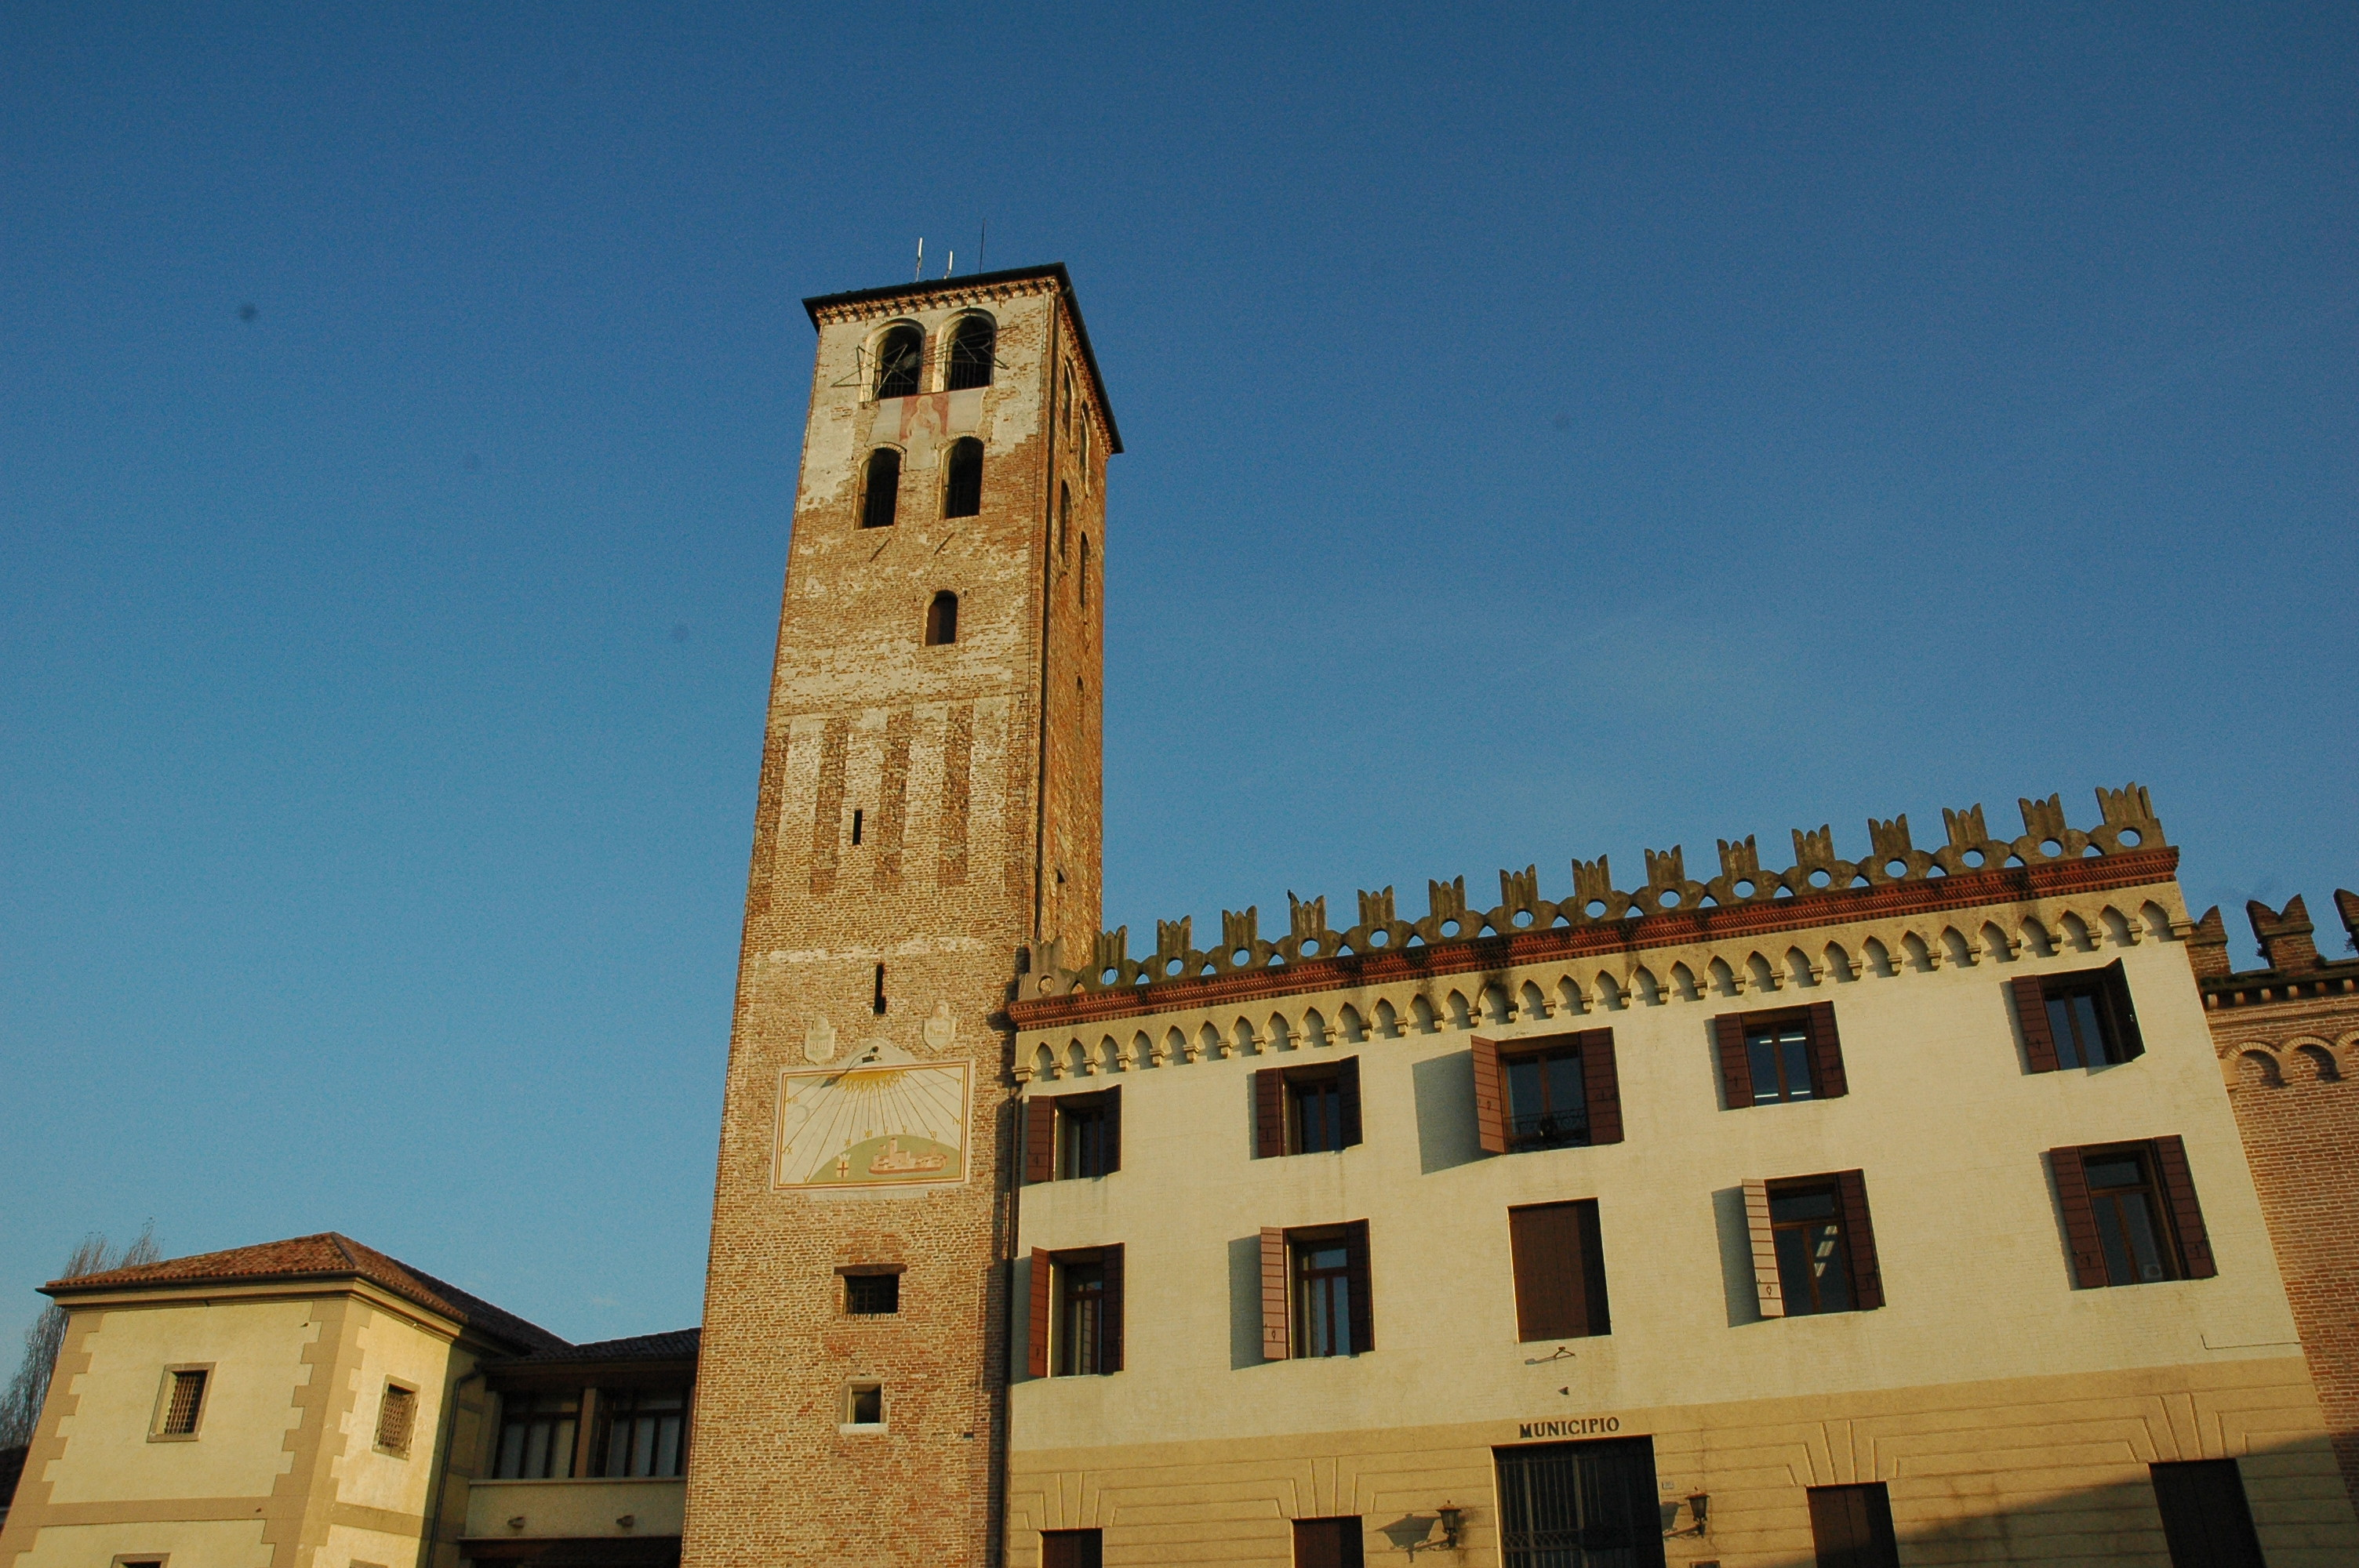
\includegraphics[width=\textwidth]{../../Project_3DAR/images/Testing/tisoDataset/img16c2.jpg}
     \end{subfigure}
     \hfill
     \begin{subfigure}[b]{0.3\textwidth}
         \centering
         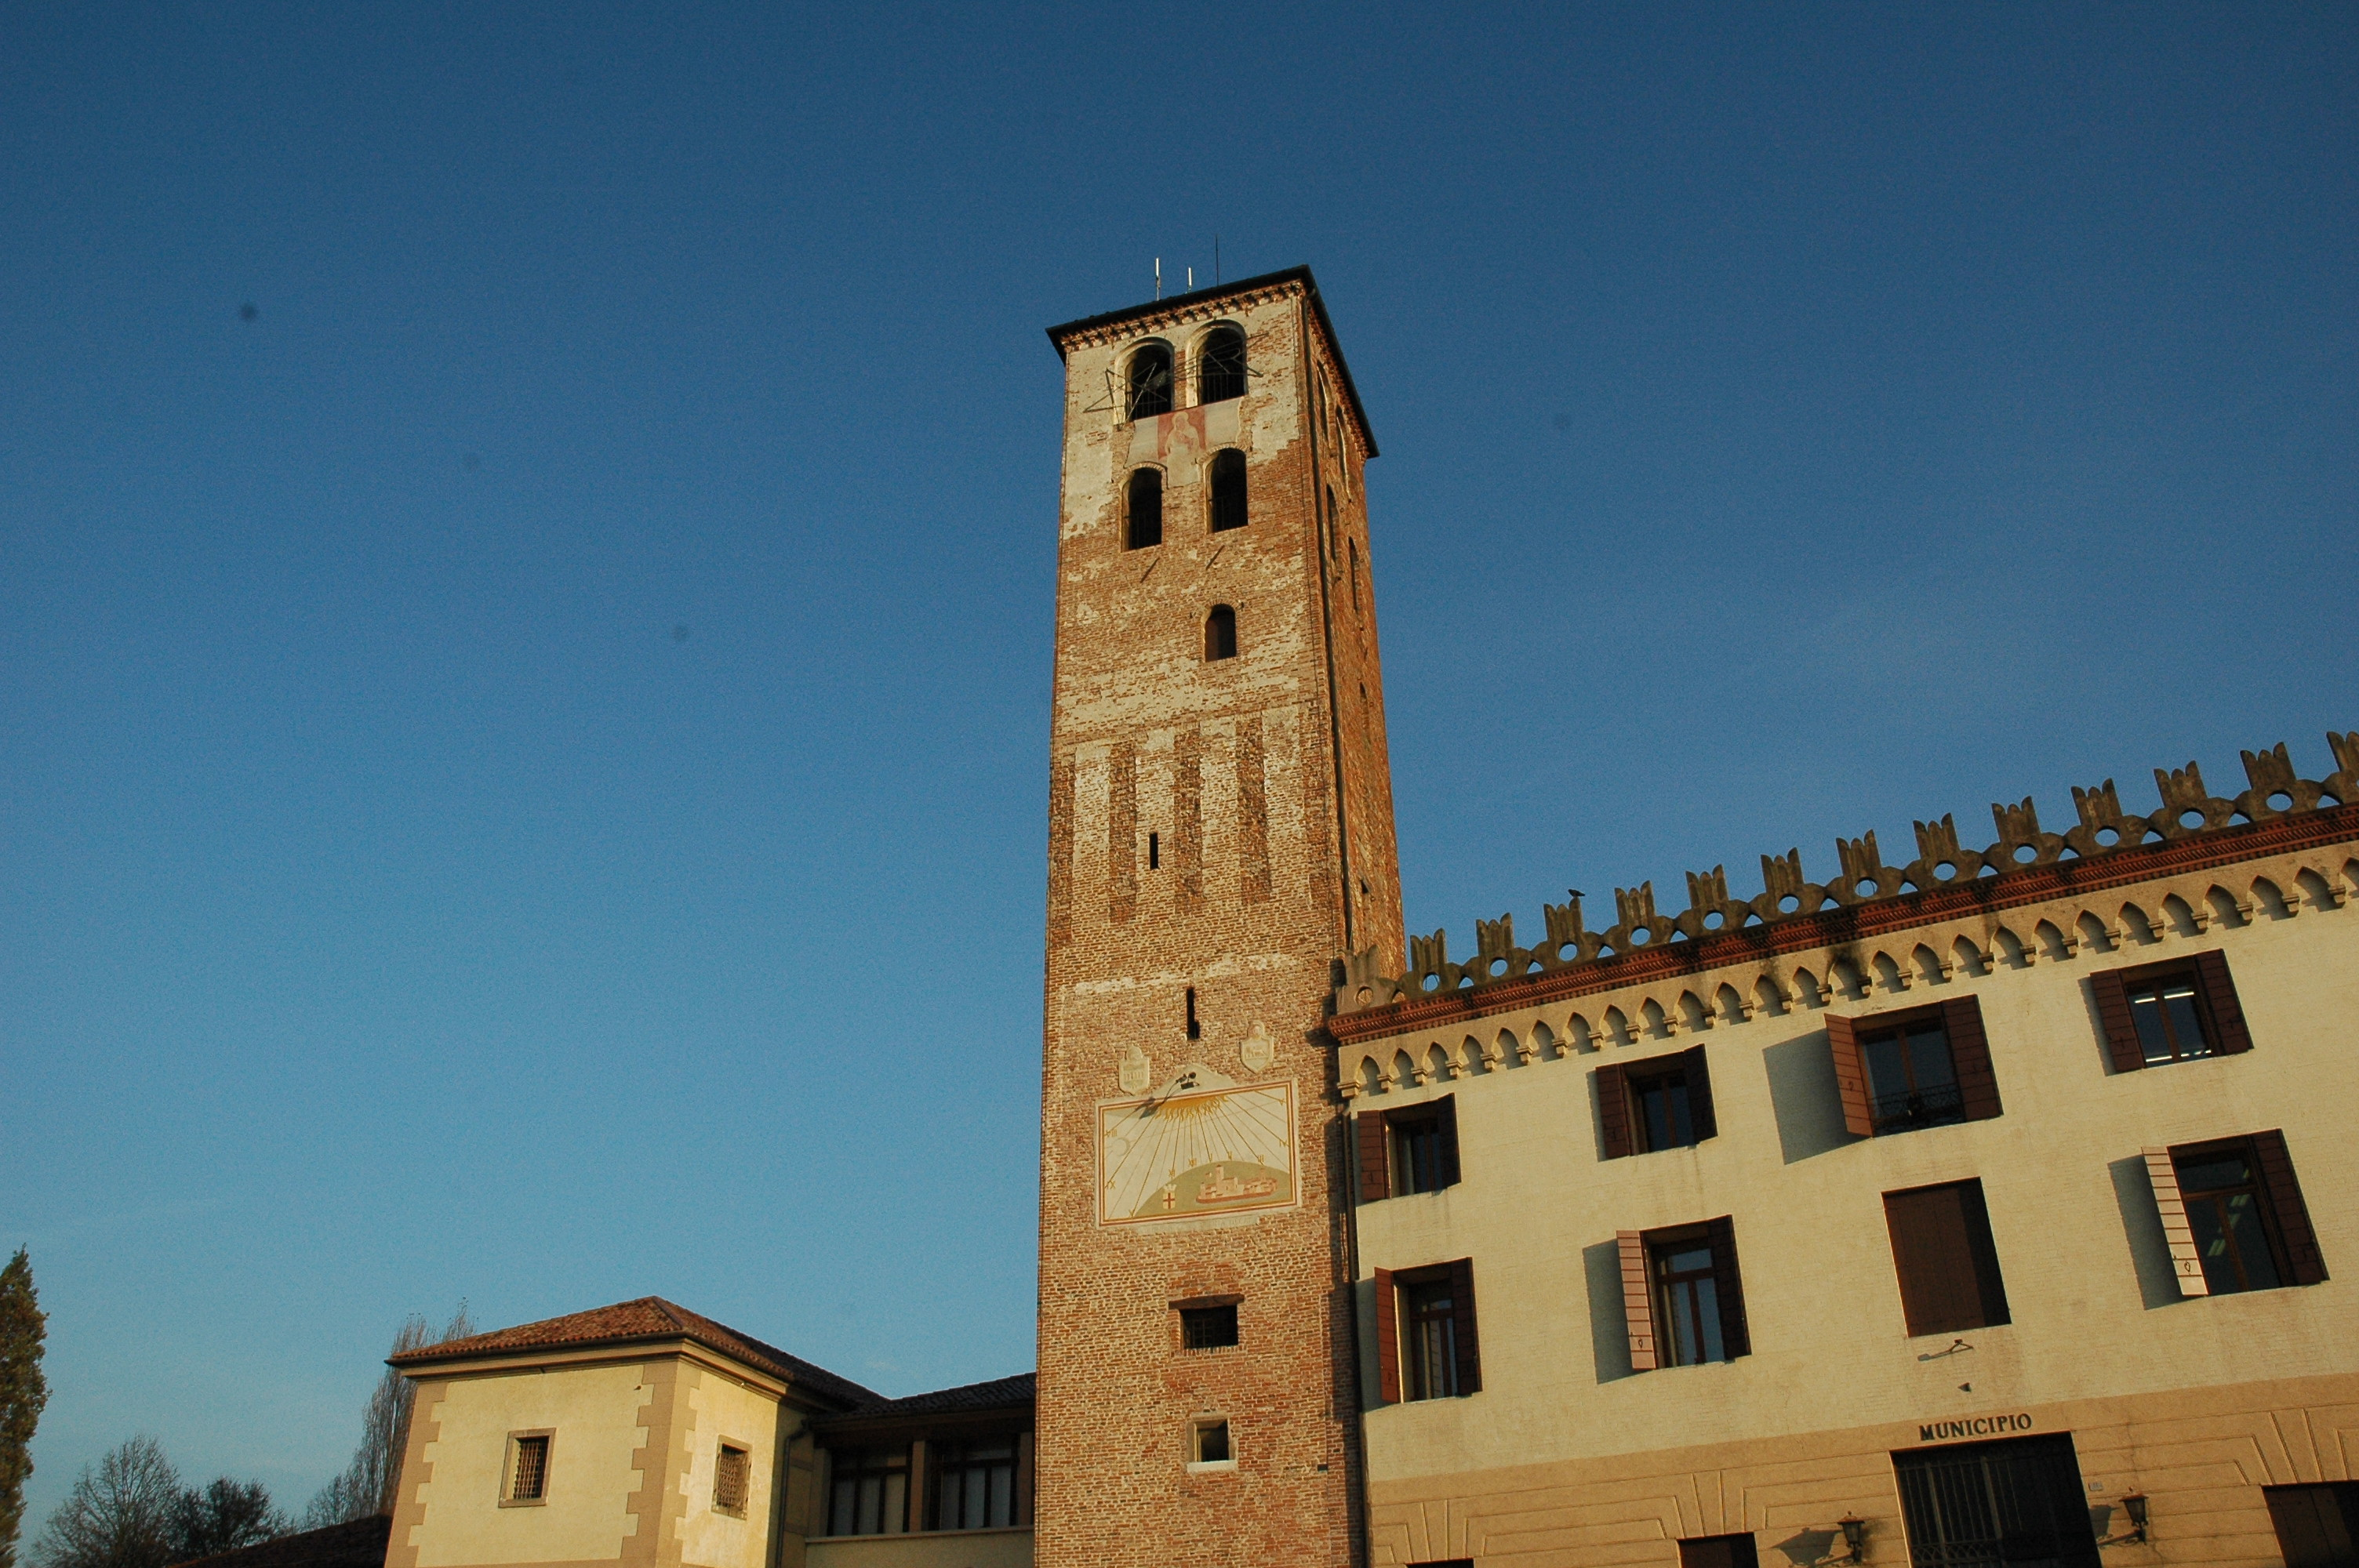
\includegraphics[width=\textwidth]{../../Project_3DAR/images/Testing/tisoDataset/img18c2.jpg}
     \end{subfigure}
     \hfill
     \begin{subfigure}[b]{0.3\textwidth}
         \centering
         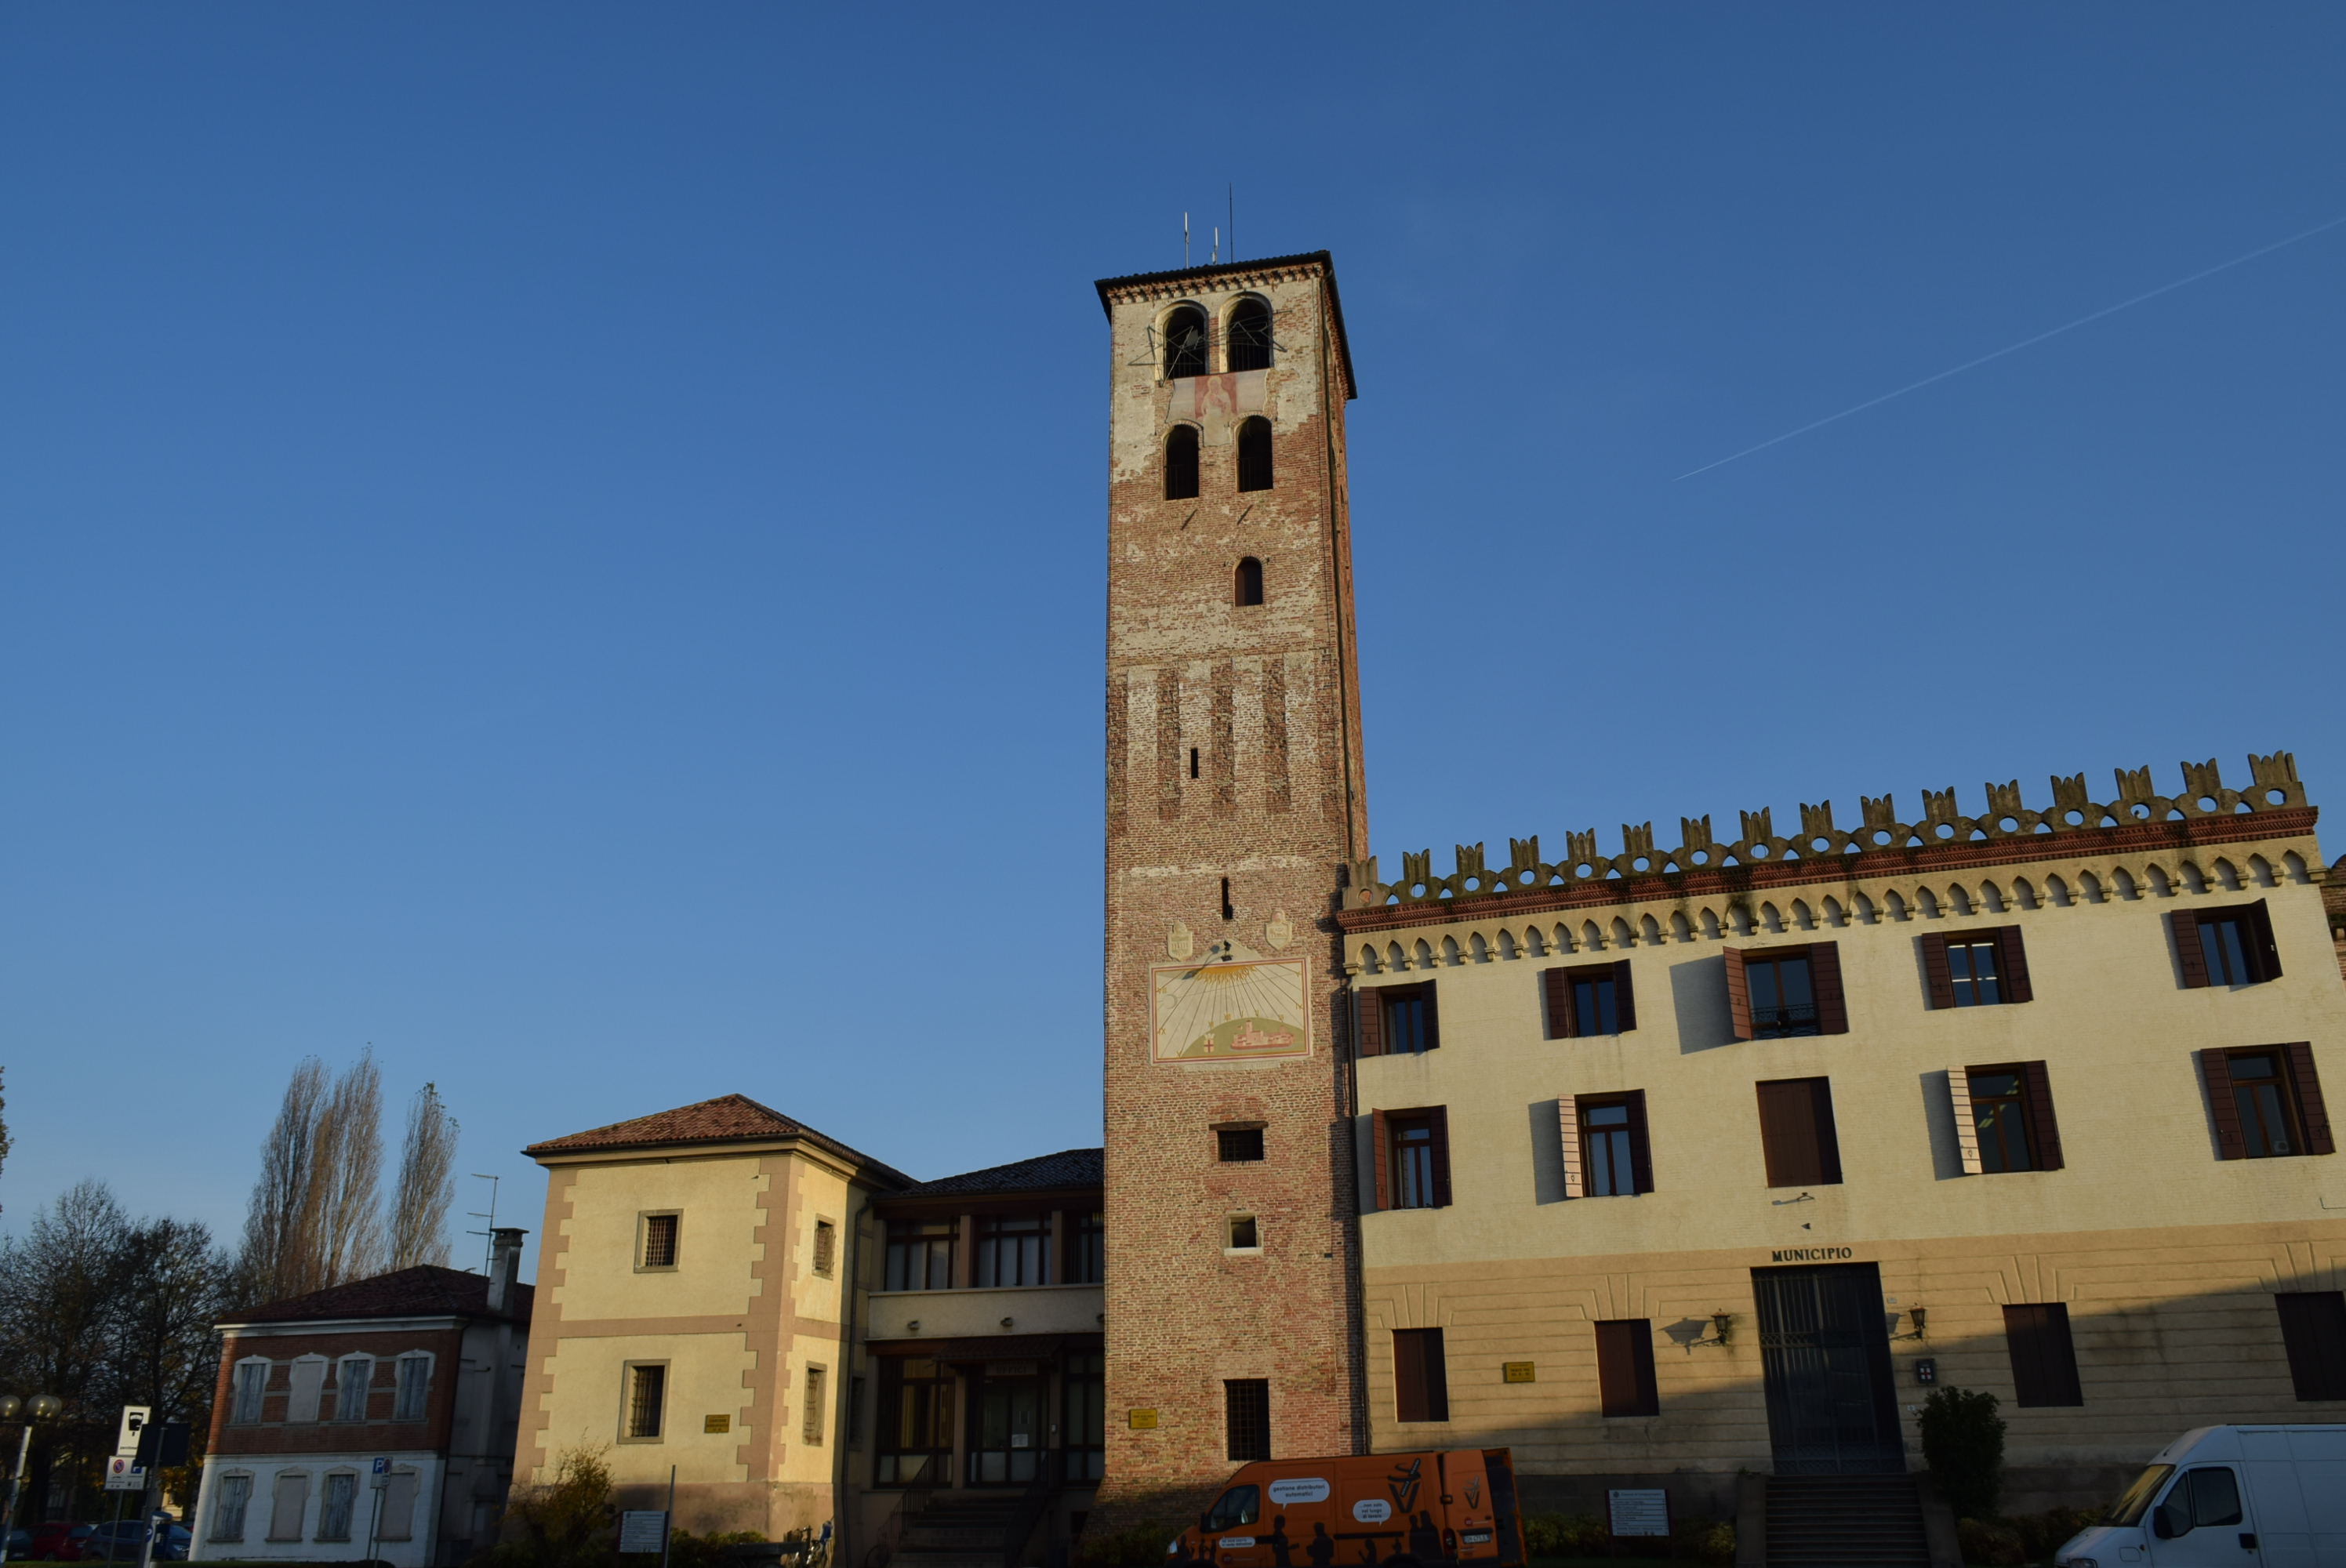
\includegraphics[width=\textwidth]{../../Project_3DAR/images/Testing/tisoDataset/img26c3.jpg}
     \end{subfigure}
        \caption{samples from Tiso dataset.}
        \label{fig:tiso}
\end{figure}



% \chapter{Research update}
 %!TeX root = ../main.tex

\section{Development}
\subsection{Training}
The images from the training set are loaded into a single image datastore. After that, a loop for each image is designed in order to:
\begin{enumerate}
\item Convert the image to grayscale;
\item Detect the SURF features (using the MATLAB function ``detectSURFFeatures'');
\item Extract the features (descriptors) using the function ``extractFeatures''. In this case they are represented as a vector of $64$ columns and $N$ rows;
\item Stack vertically the descriptors of each image in a single matrix.
\end{enumerate}
The result is a big matrix containing all the descriptors for each image in column. The autoencoder has been built using the function ``layerGraph'', which requires in input a vector ``layers'' containing the structure of the Neural Network. For this purpose, we chose the following three-layer structure:
\begin{itemize}
\item an input layer that receives features of dimension 64 (using \\ ``featureInputLayer(64)'');
\item two fully connected layers of dimension 6 and 64 (using ``fullyConnectedLayer(6)'' and ``fullyConnectedLayer(64)''), the second one having dimension 64 as will work as output layer;
\item a regression layer that will predict the reconstructed values (using \\ ``regressionLayer'').
\end{itemize}
After some testing, we found out that for the inside layer a dimension of $4$ was too strict (The reconstructed values were too compressed, i.e. too far from the input ones) while for $8$ they were too close to the input ones, so we opted for the compromise of $6$.
Regarding the training options, we decided to use an \emph{adam} (Adaptive Moment Estimation) optimizer and a maximum number of epochs of 2, since even after one epoch the training loss was pretty stable around $5\%$ (fig. \ref{fig:2epochs}).

\begin{figure}[H]
    \centering
    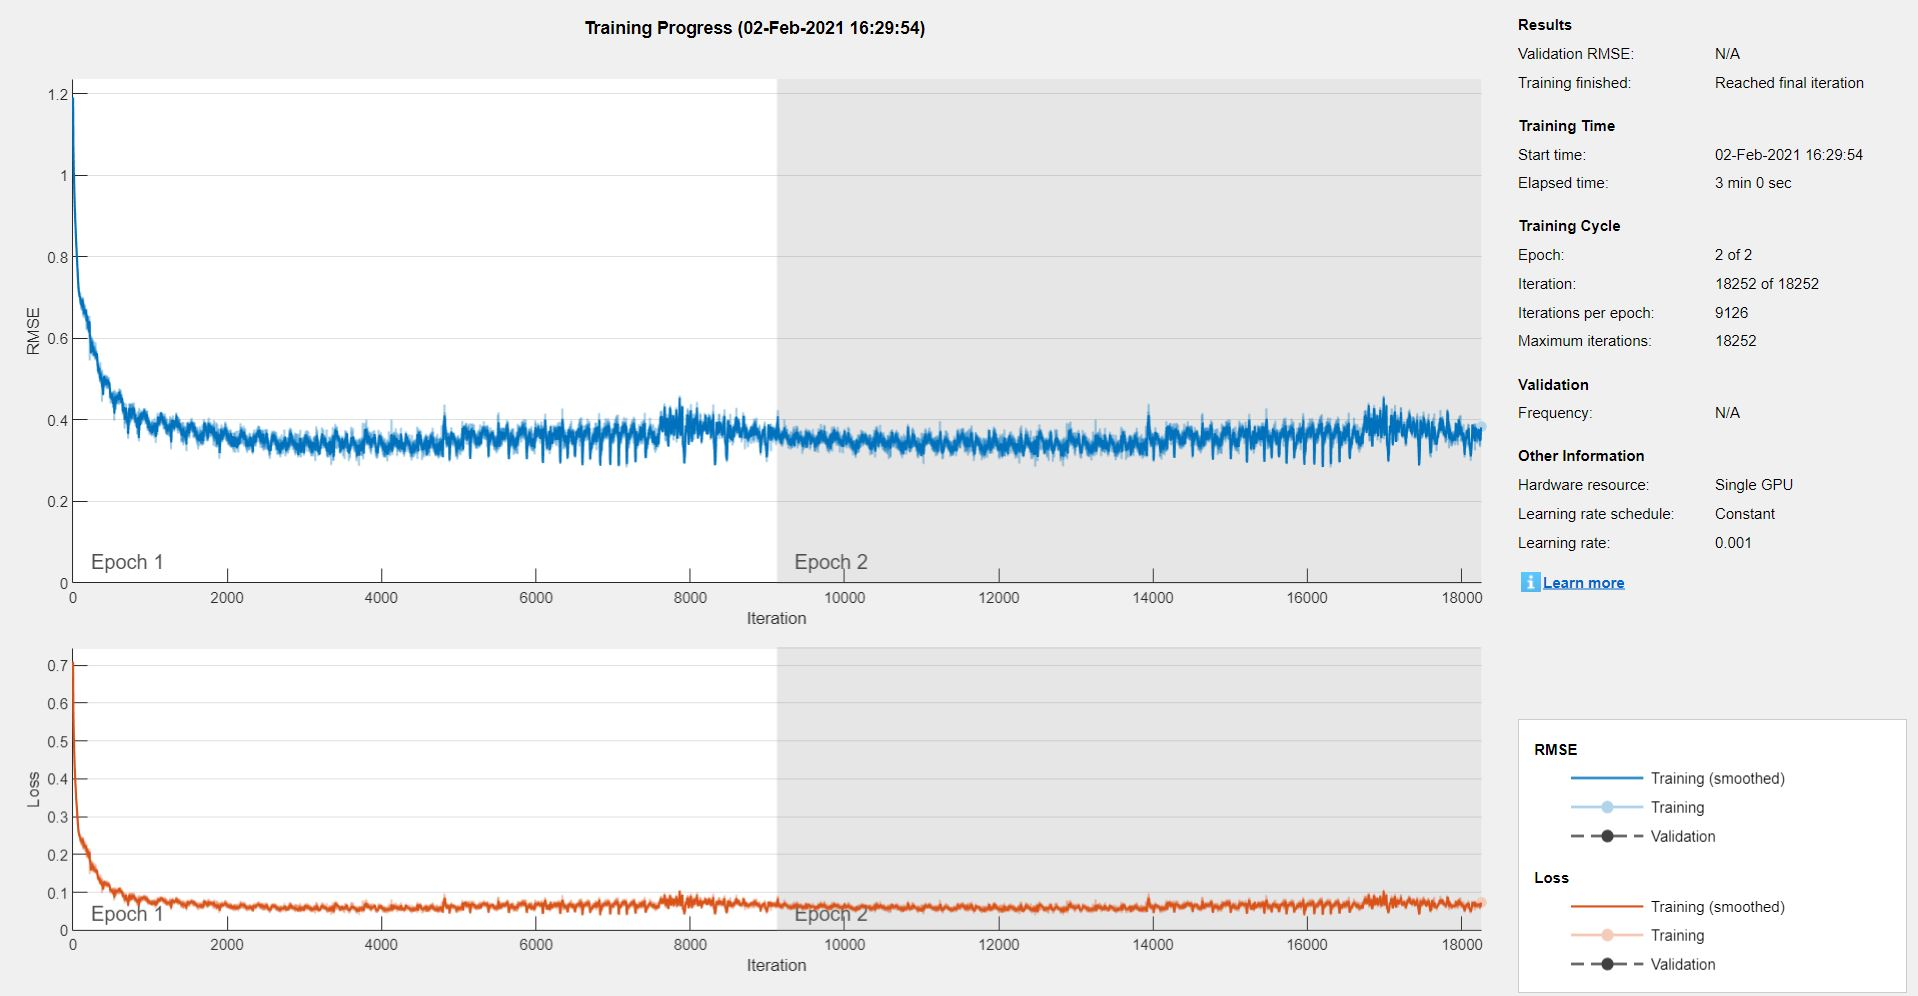
\includegraphics[width=\textwidth]{images/2EPOCHS.jpg}
    \caption{Training results after 2 epochs (18252 iterations).}
    \label{fig:2epochs}    
\end{figure}

The autoencoder is then succesfully trained (using the function ``trainNetwork'') in order to be ready to be used for the testing phase. A useful trick in order to fasten up the operation of testing and not doing everytime the training (which could require some time if the number of epochs is increased) is to save the workspace at the end of the training section and load it at the beginning of the testing one, so that everytime that section is called the autoencoder will remain trained just like it was the first time.

\subsection{Testing}
For the phase of testing the image datasets must be loaded separately (one for each building). To be clearer, this section simply called two functions, one for the features extraction, and one for the matchings calculations. This was done because COLMAP requires specific type of files in order to perform a reconstruction (will be better explained in sec. \ref{sec:COLMAP}).

\subsubsection{Function FEATURES} \label{sec:FEATURES}
This function aims to reconstruct the features of each image with the autoencoder and the original ones in a .txt file for each image in the form ``location\_x location\_y scale orientation'' followed by 128 zeros since COLMAP works with SIFT features, which are of that size.
The workflow of the function is the following:
\begin{itemize}
\item The path containing the features is cleaned from older files containing the features;
\item For each image in the image datastore considered, which is given in input along with the autoencoder:
\begin{enumerate}
\item The image is converted to grayscale;
\item The features are detected and then extracted like for the phase of training, only this time they won't be stacked in a single matrix but the features \textbf{extracted} are going to be fed into the autoencoder and be returned from the function while the \textbf{detected} ones are going to be divided in Location, Scale, Orientation in order to be printed in a .txt file of the form
\begin{align*}
& N\ 128 \\
& location_{x0} \ location_{y0} \ scale_0 \ orientation_0 \ 0\  ... (x128)\  0 \\
& location_{x1} \ location_{y1} \ scale_1 \ orientation_1 \ 0\  ... (x128)\  0 \\
& ... \\
& location_{xN} \ location_{yN} \ scale_N \ orientation_N \ 0\  ... (x128)\  0 \\
\end{align*}  
where $N$ is the number of features.
\end{enumerate} 
\end{itemize}

\subsubsection{Function MATCHINGS} \label{sec:MATCHINGS}
The function, given in input the image datastore considered and the features (compressed or not) matches the features of each couple of image $i,j$. To avoid repetitions ($i,j$ and $j,i$ have the same matchings) the MATLAB function ``matchFeatures'' is called for every $i,j$ for $i$ going from 1 to the last feature -1 and $j$ going from $i+1$ to the last feature. The matchings are all stacked in a single .txt file of the form:
\begin{align*}
& image0.jpg\ image1.jpg \\
& matching1_0\ matching1_1 \\
& matching2_0\ matching2_1 \\
& ... \\
& matchingN_0\ matchingN_1 \\
& \\
& image0.jpg\ image2.jpg \\
& matching1_0\ matching1_2 \\
& ...
\end{align*}  

 % \chapter{Some chapter}
 %!TeX root = ../main.tex

\section{COLMAP} \label{sec:COLMAP}
Having all the required files the performances of the compression system can be tested on a 3D-Reconstruction software, like COLMAP (\url{https://colmap.github.io/}). This software was meant for using SIFT features (see fig. \ref{fig:descriptors}), which are heavier and more performing in terms of quality but also less robust to image transformations (which must be accounted since the images are taken with a mobile phone) and patented. A trick that can be used is to use SURF features (64 float) and faking a larger dimensionality (128 float) by adding zeros. This way COLMAP recognizes the right dimensionality of the files while using SURF features instead of SIFT. In order to start the reconstruction, COLMAP will need three things:
\begin{enumerate}
\item A database to store the informations;
\item A set of images of the same scenario in different perspectives;
\item A .txt file for each image containing the features, in the format specified in sec. \ref{sec:FEATURES}. The title of the file must be the name of the image followed by .txt (\emph{e.g: image001.jpg.txt});
\item A .txt file containing the matchings between each image in the format specified in sec. \ref{sec:MATCHINGS}.
\end{enumerate}
Not having these will result in an error inside COLMAP which won't start the reconstruction.


\begin{figure}[h!]
    \centering
    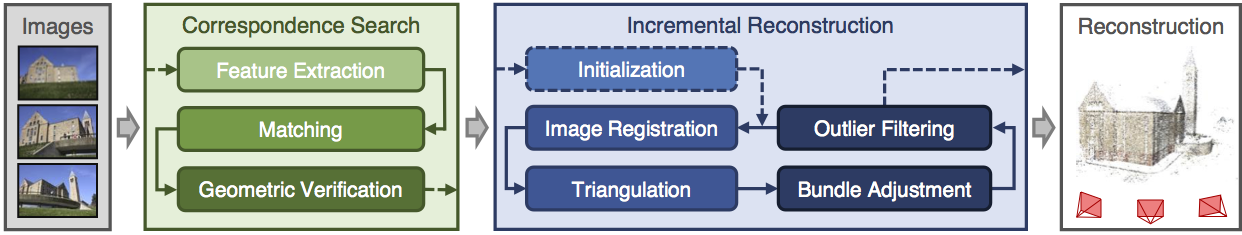
\includegraphics[width=\textwidth]{images/colmap.png}
    \caption{COLMAP’s incremental SfM pipeline.}
    \label{fig:colmap}    
\end{figure}
 
% \chapter{Planning and Conclusion}
 %!TeX root = ../main.tex


\section{Conclusions}
By performing a reconstruction in COLMAP, a final result is obtained and in this case, as shown in fig. \ref{fig:fountaintrue} and \ref{fig:tisotrue}, the fountain is rebuilt in a more sparse form due to the smaller amount of information provided to the software. In fact, from the statistics, there is a mean of observations per image equal to 4751.36 and a total number of observations equal to 52256. The data are almost a third lower than those obtained with the SURF algorithm without using the compression of the descriptors. Fig. \ref{fig:fountainautoenc} and \ref{fig:tisoautoenc} refers precisely to the final result without the use of the autoencoder and therefore all the features and matchings obtained by the SURF algorithm are supplied to COLMAP without regression. Comparing the two results, significant differences are visible in the reconstruction quality of the fountain.


\begin{figure}[H]
     \centering
     \begin{subfigure}[b]{.5\textwidth}
		\centering
		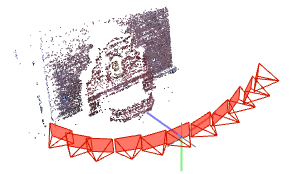
\includegraphics[width=\textwidth]{images/fountainautoenc.png}  
		\caption{\centering Fountain reconstructed with the autoencoder.}
	    	\label{fig:fountainautoenc} 
     \end{subfigure}
     \hfill
     \begin{subfigure}[b]{0.49\textwidth}
		\centering
    		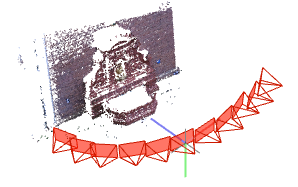
\includegraphics[width=\textwidth]{images/fountaintrue.png}
		\caption{\centering Fountain reconstructed without the autoencoder.}
		\label{fig:fountaintrue}   
     \end{subfigure}
        \caption{Fountain reconstruction using COLMAP.}
        \label{fig:fountain3D}
\end{figure}


\begin{figure}[H]
     \centering
          \begin{subfigure}[b]{0.5\textwidth}
		\centering
    		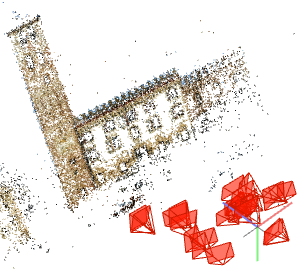
\includegraphics[width=\textwidth]{images/tisoautoenc.png}
		\caption{\centering Tiso reconstructed with the autoencoder.}
		\label{fig:tisoautoenc}   
     \end{subfigure}
     \hfill
     \begin{subfigure}[b]{.49\textwidth}
		\centering
		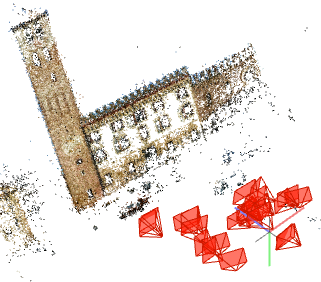
\includegraphics[width=\textwidth]{images/tisotrue.png}  
		\caption{\centering Tiso reconstructed without the autoencoder.}
	    	\label{fig:tisotrue} 
     \end{subfigure}
        \caption{Tiso reconstruction using COLMAP.}
        \label{fig:Tiso3D}
\end{figure}


This type of compression can be useful in environments where the quality of reconstruction is not important, for example in object detection, where is not crucial to exactly reconstruct the object with respect to the detection result ``true/false''. In can be seen from the compressed images that the edges of the objects are mostly preserved while straight planes are ``thinned out'', i.e. represented with less points.
 
 %!TeX root = ../main.tex
\section{MATLAB Code}

\lstinputlisting{../PROJECT_3DAR_2.m}


    
% Include appendix      % Set this up if needed
%\appendix

% Insert bibliography here
%\printbibliography

\end{document}

% End of document
%-----------------------------------------------------------------------------------------------------